\PassOptionsToPackage{unicode=true}{hyperref} % options for packages loaded elsewhere
\PassOptionsToPackage{hyphens}{url}
\PassOptionsToPackage{dvipsnames,svgnames*,x11names*}{xcolor}
%
\documentclass[]{article}
\usepackage{lmodern}
\usepackage{amssymb,amsmath}
\usepackage{ifxetex,ifluatex}
\usepackage{fixltx2e} % provides \textsubscript
\ifnum 0\ifxetex 1\fi\ifluatex 1\fi=0 % if pdftex
  \usepackage[T1]{fontenc}
  \usepackage[utf8]{inputenc}
  \usepackage{textcomp} % provides euro and other symbols
\else % if luatex or xelatex
  \usepackage{unicode-math}
  \defaultfontfeatures{Ligatures=TeX,Scale=MatchLowercase}
\fi
% use upquote if available, for straight quotes in verbatim environments
\IfFileExists{upquote.sty}{\usepackage{upquote}}{}
% use microtype if available
\IfFileExists{microtype.sty}{%
\usepackage[]{microtype}
\UseMicrotypeSet[protrusion]{basicmath} % disable protrusion for tt fonts
}{}
\IfFileExists{parskip.sty}{%
\usepackage{parskip}
}{% else
\setlength{\parindent}{0pt}
\setlength{\parskip}{6pt plus 2pt minus 1pt}
}
\usepackage{xcolor}
\usepackage{hyperref}
\hypersetup{
            pdftitle={Pre-Analysis Plan: Give a Little, Take a Little. Political Parties' Reputational Cost of Compromise},
            colorlinks=true,
            linkcolor=blue,
            filecolor=Maroon,
            citecolor=Blue,
            urlcolor=blue,
            breaklinks=true}
\urlstyle{same}  % don't use monospace font for urls
\usepackage[margin=1in]{geometry}
\usepackage{color}
\usepackage{fancyvrb}
\newcommand{\VerbBar}{|}
\newcommand{\VERB}{\Verb[commandchars=\\\{\}]}
\DefineVerbatimEnvironment{Highlighting}{Verbatim}{commandchars=\\\{\}}
% Add ',fontsize=\small' for more characters per line
\usepackage{framed}
\definecolor{shadecolor}{RGB}{248,248,248}
\newenvironment{Shaded}{\begin{snugshade}}{\end{snugshade}}
\newcommand{\AlertTok}[1]{\textcolor[rgb]{0.94,0.16,0.16}{#1}}
\newcommand{\AnnotationTok}[1]{\textcolor[rgb]{0.56,0.35,0.01}{\textbf{\textit{#1}}}}
\newcommand{\AttributeTok}[1]{\textcolor[rgb]{0.77,0.63,0.00}{#1}}
\newcommand{\BaseNTok}[1]{\textcolor[rgb]{0.00,0.00,0.81}{#1}}
\newcommand{\BuiltInTok}[1]{#1}
\newcommand{\CharTok}[1]{\textcolor[rgb]{0.31,0.60,0.02}{#1}}
\newcommand{\CommentTok}[1]{\textcolor[rgb]{0.56,0.35,0.01}{\textit{#1}}}
\newcommand{\CommentVarTok}[1]{\textcolor[rgb]{0.56,0.35,0.01}{\textbf{\textit{#1}}}}
\newcommand{\ConstantTok}[1]{\textcolor[rgb]{0.00,0.00,0.00}{#1}}
\newcommand{\ControlFlowTok}[1]{\textcolor[rgb]{0.13,0.29,0.53}{\textbf{#1}}}
\newcommand{\DataTypeTok}[1]{\textcolor[rgb]{0.13,0.29,0.53}{#1}}
\newcommand{\DecValTok}[1]{\textcolor[rgb]{0.00,0.00,0.81}{#1}}
\newcommand{\DocumentationTok}[1]{\textcolor[rgb]{0.56,0.35,0.01}{\textbf{\textit{#1}}}}
\newcommand{\ErrorTok}[1]{\textcolor[rgb]{0.64,0.00,0.00}{\textbf{#1}}}
\newcommand{\ExtensionTok}[1]{#1}
\newcommand{\FloatTok}[1]{\textcolor[rgb]{0.00,0.00,0.81}{#1}}
\newcommand{\FunctionTok}[1]{\textcolor[rgb]{0.00,0.00,0.00}{#1}}
\newcommand{\ImportTok}[1]{#1}
\newcommand{\InformationTok}[1]{\textcolor[rgb]{0.56,0.35,0.01}{\textbf{\textit{#1}}}}
\newcommand{\KeywordTok}[1]{\textcolor[rgb]{0.13,0.29,0.53}{\textbf{#1}}}
\newcommand{\NormalTok}[1]{#1}
\newcommand{\OperatorTok}[1]{\textcolor[rgb]{0.81,0.36,0.00}{\textbf{#1}}}
\newcommand{\OtherTok}[1]{\textcolor[rgb]{0.56,0.35,0.01}{#1}}
\newcommand{\PreprocessorTok}[1]{\textcolor[rgb]{0.56,0.35,0.01}{\textit{#1}}}
\newcommand{\RegionMarkerTok}[1]{#1}
\newcommand{\SpecialCharTok}[1]{\textcolor[rgb]{0.00,0.00,0.00}{#1}}
\newcommand{\SpecialStringTok}[1]{\textcolor[rgb]{0.31,0.60,0.02}{#1}}
\newcommand{\StringTok}[1]{\textcolor[rgb]{0.31,0.60,0.02}{#1}}
\newcommand{\VariableTok}[1]{\textcolor[rgb]{0.00,0.00,0.00}{#1}}
\newcommand{\VerbatimStringTok}[1]{\textcolor[rgb]{0.31,0.60,0.02}{#1}}
\newcommand{\WarningTok}[1]{\textcolor[rgb]{0.56,0.35,0.01}{\textbf{\textit{#1}}}}
\usepackage{graphicx,grffile}
\makeatletter
\def\maxwidth{\ifdim\Gin@nat@width>\linewidth\linewidth\else\Gin@nat@width\fi}
\def\maxheight{\ifdim\Gin@nat@height>\textheight\textheight\else\Gin@nat@height\fi}
\makeatother
% Scale images if necessary, so that they will not overflow the page
% margins by default, and it is still possible to overwrite the defaults
% using explicit options in \includegraphics[width, height, ...]{}
\setkeys{Gin}{width=\maxwidth,height=\maxheight,keepaspectratio}
\setlength{\emergencystretch}{3em}  % prevent overfull lines
\providecommand{\tightlist}{%
  \setlength{\itemsep}{0pt}\setlength{\parskip}{0pt}}
\setcounter{secnumdepth}{5}
% Redefines (sub)paragraphs to behave more like sections
\ifx\paragraph\undefined\else
\let\oldparagraph\paragraph
\renewcommand{\paragraph}[1]{\oldparagraph{#1}\mbox{}}
\fi
\ifx\subparagraph\undefined\else
\let\oldsubparagraph\subparagraph
\renewcommand{\subparagraph}[1]{\oldsubparagraph{#1}\mbox{}}
\fi

% set default figure placement to htbp
\makeatletter
\def\fps@figure{htbp}
\makeatother

\usepackage{floatrow}
\floatsetup[figure]{capposition=top}
\floatsetup[table]{capposition=top}
\usepackage{booktabs}
\usepackage{graphicx}
\usepackage{amsmath}
\usepackage{longtable}
\usepackage{array}
\usepackage{multirow}
\usepackage{wrapfig}
\usepackage{float}
\usepackage{colortbl}
\usepackage{pdflscape}
\usepackage{tabu}
\usepackage{threeparttable}
\usepackage{threeparttablex}
\usepackage[normalem]{ulem}
\usepackage{makecell}
\usepackage{xcolor}
\usepackage[utf8]{inputenc}
\usepackage{booktabs}
\usepackage{longtable}
\usepackage{array}
\usepackage{multirow}
\usepackage{wrapfig}
\usepackage{float}
\usepackage{colortbl}
\usepackage{pdflscape}
\usepackage{tabu}
\usepackage{threeparttable}
\usepackage{threeparttablex}
\usepackage[normalem]{ulem}
\usepackage{makecell}
\usepackage{xcolor}

\title{Pre-Analysis Plan: Give a Little, Take a Little. Political Parties'
Reputational Cost of Compromise}
\author{}
\date{\vspace{-2.5em}16 October, 2021 - 12:31:00 (CEST)}

\begin{document}
\maketitle

{
\hypersetup{linkcolor=}
\setcounter{tocdepth}{2}
\tableofcontents
}
\newpage

\hypertarget{expectations}{%
\section{Expectations}\label{expectations}}

\textbf{Steadfast hypothesis} (\emph{H1}): All else equal, in-partisans
view their party more positively when a party remains steadfast in
coalition talks, compared to accepting a compromise.

\textbf{Outcome hypothesis} (\emph{H2}): All else equal, in-partisans
view their party more positively when coalition talks continue compared
to stalling of the coalition talks.

\textbf{Compromise hypothesis} (\emph{H3}): All else equal, in-partisans
view their party that accepts a compromise more positively when
coalition talks continue compared to stalling of the coalition talks.

\textbf{Principled hypothesis} (\emph{H4}): All else equal, the more
principled a respondent is, the higher the evaluation of a steadfast
party.

\textbf{Mutual Trust hypothesis} (\emph{H5}): All else equal, the more
distrusting a respondent is, the higher the evaluation of a steadfast
party.

\hypertarget{research-desing-and-protocol}{%
\section{Research Desing and
Protocol}\label{research-desing-and-protocol}}

\hypertarget{sample}{%
\subsection{Sample}\label{sample}}

We will conduct the survey experiment in Germany in October 2021 --
approximately three weeks after the general elections of 26 September
2021. The sample, recruited through
\href{https://www.respondi.com/EN/}{Respondi}, will consist of 8,000
participants (based on the power analysis presented in Figure
\ref{fig:power}) of 18 years and older. Respondi works with opt-in
respondents, so we have implemented quota on age, gender, and education.
Moreover, we measure some more demographic background variables (see
\protect\hyperlink{control-variables}{Section 3.2}). Balance checks will
be conducted to demonstrate whether certain categories are over
represented in a certain experimental group. The study has been approved
by the
\href{https://fsw.vu.nl/nl/onderzoek/research-ethics-review/index.aspx}{Research
Ethics Review Committee} of the \textit{Vrije Universiteit Amsterdam}
(see the approval \href{LINK}{here}). To ensure good quality of our
data, two attention checks (discussed in more detail in
\protect\hyperlink{attention-checks}{Section 3.3}) are included. Each
respondent failing the attention check will be excluded and replaced
with another `good' response.

I will conduct this survey experiment in the Netherlands in April 2021.
The sample, recruited through
\href{https://www.kieskompas.nl/en/}{KiesKompas}, will consist of 2,000
participants (based on the power analysis presented in Figure
\ref{fig:power1}) of 18 years and older. Kieskompas works with
non-random opt-in respondents. Therefore, I measure many demographic
background variables (see \protect\hyperlink{control-variables}{Section
3.2}). Balance checks will be conducted to demonstrate whether certain
categories are over represented in a certain experimental group. The
study has been approved by the
\href{https://fsw.vu.nl/nl/onderzoek/research-ethics-review/index.aspx}{Research
Ethics Review Committee} of the \emph{Vrije Universiteit Amsterdam} (see
the approval
\href{https://github.com/MarikenvdVelden/willingness-to-accept-compromises/blob/main/docs/RERC_VU_compromises.pd}{here}).
To ensure good quality of our data, two attention checks (discussed in
more detail in \protect\hyperlink{attention-checks}{Section 3.3}) are
included. Each respondent failing the attention check will be excluded
and replaced with another `good' response.

\hypertarget{experimental-protocol}{%
\subsection{Experimental Protocol}\label{experimental-protocol}}

The study is conducted online and in German Participants are told that
they are taking part in a survey to get an overview of how German people
form their views on politics. After reading an informed consent message
participants are forwarded to the main questionnaire (or the survey will
be terminated if they do not agree to the consent form).

First, participants complete a set of demographic variables
(i.e.~income, employment, and degree of urbanization). This block ends
with one of the two attention checks included in this survey. When
participants fail this attention check, a warning appears asking them to
read the question again carefully and to answer again. Thereafter, a set
of background variables are asked on their stances on the political
issues, some are used in the experiment (i.e.~top tax, speed limit,
education, legalization of Cannabis), their political interest and
knowledge, as well as on their ideological position -- the full codeboek
can be viewed \protect\hyperlink{}{here}. Next, participants are forced
to choose between one of four parties -- CDU, SPD, Greens, or FDP -- as
their in-party. To account for variation of in-party strength,
respondents are surveyed on this too. Before entering the experimental
condition, respondents get a second attention check. Only when they have
answered it correctly, they enter the first round of the experiment --
if they fail to answer the question correctly, they are thrown out of
the survey. After the experimental treatment, the heterogeneous
treatments (principledness and mutual trust) and a post-treatmnet
question (populist attitudes) are asked.

The stimuli in the experiment are Instagram-posts in the same style as
the German political parties:
\href{https://www.instagram.com/cdu}{CDU},\href{https://www.instagram.com/die_gruenen}{Greens},
\href{https://www.instagram.com/fdp}{FDP},
\href{https://www.instagram.com/spdde}{SPD}. We follow Munger et al.
{[}CITE{]}'s reasoning: Given that people are more used to receiving
political information from social media, these short messages are more
common and capture people's attention better. However, to account for
age differences, we have put a press release message on the site of the
post (see Figure \ref{fig:treatment_example}). In these messages, we
manipulate: a) the \emph{potential coalition parter} of the party (SPD
and the Greens for CDU or FDP, CDU and FDP for SPD and the Greens); b)
whether or not a party is \emph{steadfast} or \emph{willing to
compromise}; and c) whether the coalition talks are \emph{stalled or
continue}. This creates a full \texttt{2*2*2} factorial experiment --
whereas the first manipulation is in-build to mimic reality, and will be
controlled for in the analyses, but does not play a role in the
hypotheses testing. For an illustration of the stimulus material, see
Figure \ref{fig:treatment_example}.

\begin{figure}

{\centering 
\includegraphics[width=0.85\linewidth]{/Users/marikenvandervelden/Dropbox/Papers/veni_project_mm/willingness-to-accept-compromises/docs/pre-analysis-plan/example_treatment} 

}

\caption{\label{fig:treatment_example}Example of Stimulus Material}\label{fig:treatment-example}
\end{figure}

\hypertarget{power-analysis}{%
\subsection{Power Analysis}\label{power-analysis}}

As detailed in \protect\hyperlink{analysis}{Section 4}, we conduct an
OLS regression for each of the dependent variables: a) trust in the
party; b) sincerity of the party; and c) representation of the party,
and the three manipulations (potential coalition partner, being
steadfast, and the outcome) as independent variables. Each hypothesis is
tested separately for the two issues. To calculate power for the
hypotheses, the R package \texttt{DeclareDesign} is used (Blair et al.
2019). Based on the study of Fortunato (2021), the effect sizes are
between \texttt{b\ =\ 0.2} and \texttt{b\ =\ 0.1} -- i.e.~a small effect
visualized by the purple and blue lines in Figure \ref{fig:power1}. The
hypothesis are directional, Figure \ref{fig:power1} therefore displays
one-tailed tests with \(\alpha\) \texttt{=\ 0.05}. The power analysis
shows that testing hypotheses 1 and 2 requires a sample size of
\texttt{4,000} participants (x-axis) to reach \texttt{95}\% power (black
dashed line, in the left-panel of Figure \ref{fig:power}). Note that if
the effect size is bigger then \texttt{0.2}, smaller sample sizes are
sufficient to reach \texttt{95\textbackslash{}\%} power. To test H3, the
combination of steadfast and outcome, we can detect an effect
\(\beta = 0.1\) (purple line) with reasonable levels of power
(\texttt{80}\%, as indicated by the gray dotted line) and a one-tailed
test of significance at \(\alpha =0.05\) with a sample of \texttt{4,000}
participants (Middle Left-Panel of Figure \ref{fig:power}). A
probability of approximately \texttt{20}\% remains for a Type II error
remains when testing Hypotheses 3. We will therefore test all hypotheses
first by issue and second, by pooling our data across issues. As the
right-hand panel of Figure \ref{fig:power} demonstrates, this will give
sufficient power -- yellow and purple lines are approximating
\texttt{100}\% with 8,000 respondents.

\begin{Shaded}
\begin{Highlighting}[]
\KeywordTok{source}\NormalTok{(here}\OperatorTok{::}\KeywordTok{here}\NormalTok{(}\StringTok{"docs/pre-analysis-plan/poweranalysis.R"}\NormalTok{))}
\end{Highlighting}
\end{Shaded}

\begin{figure}

{\centering 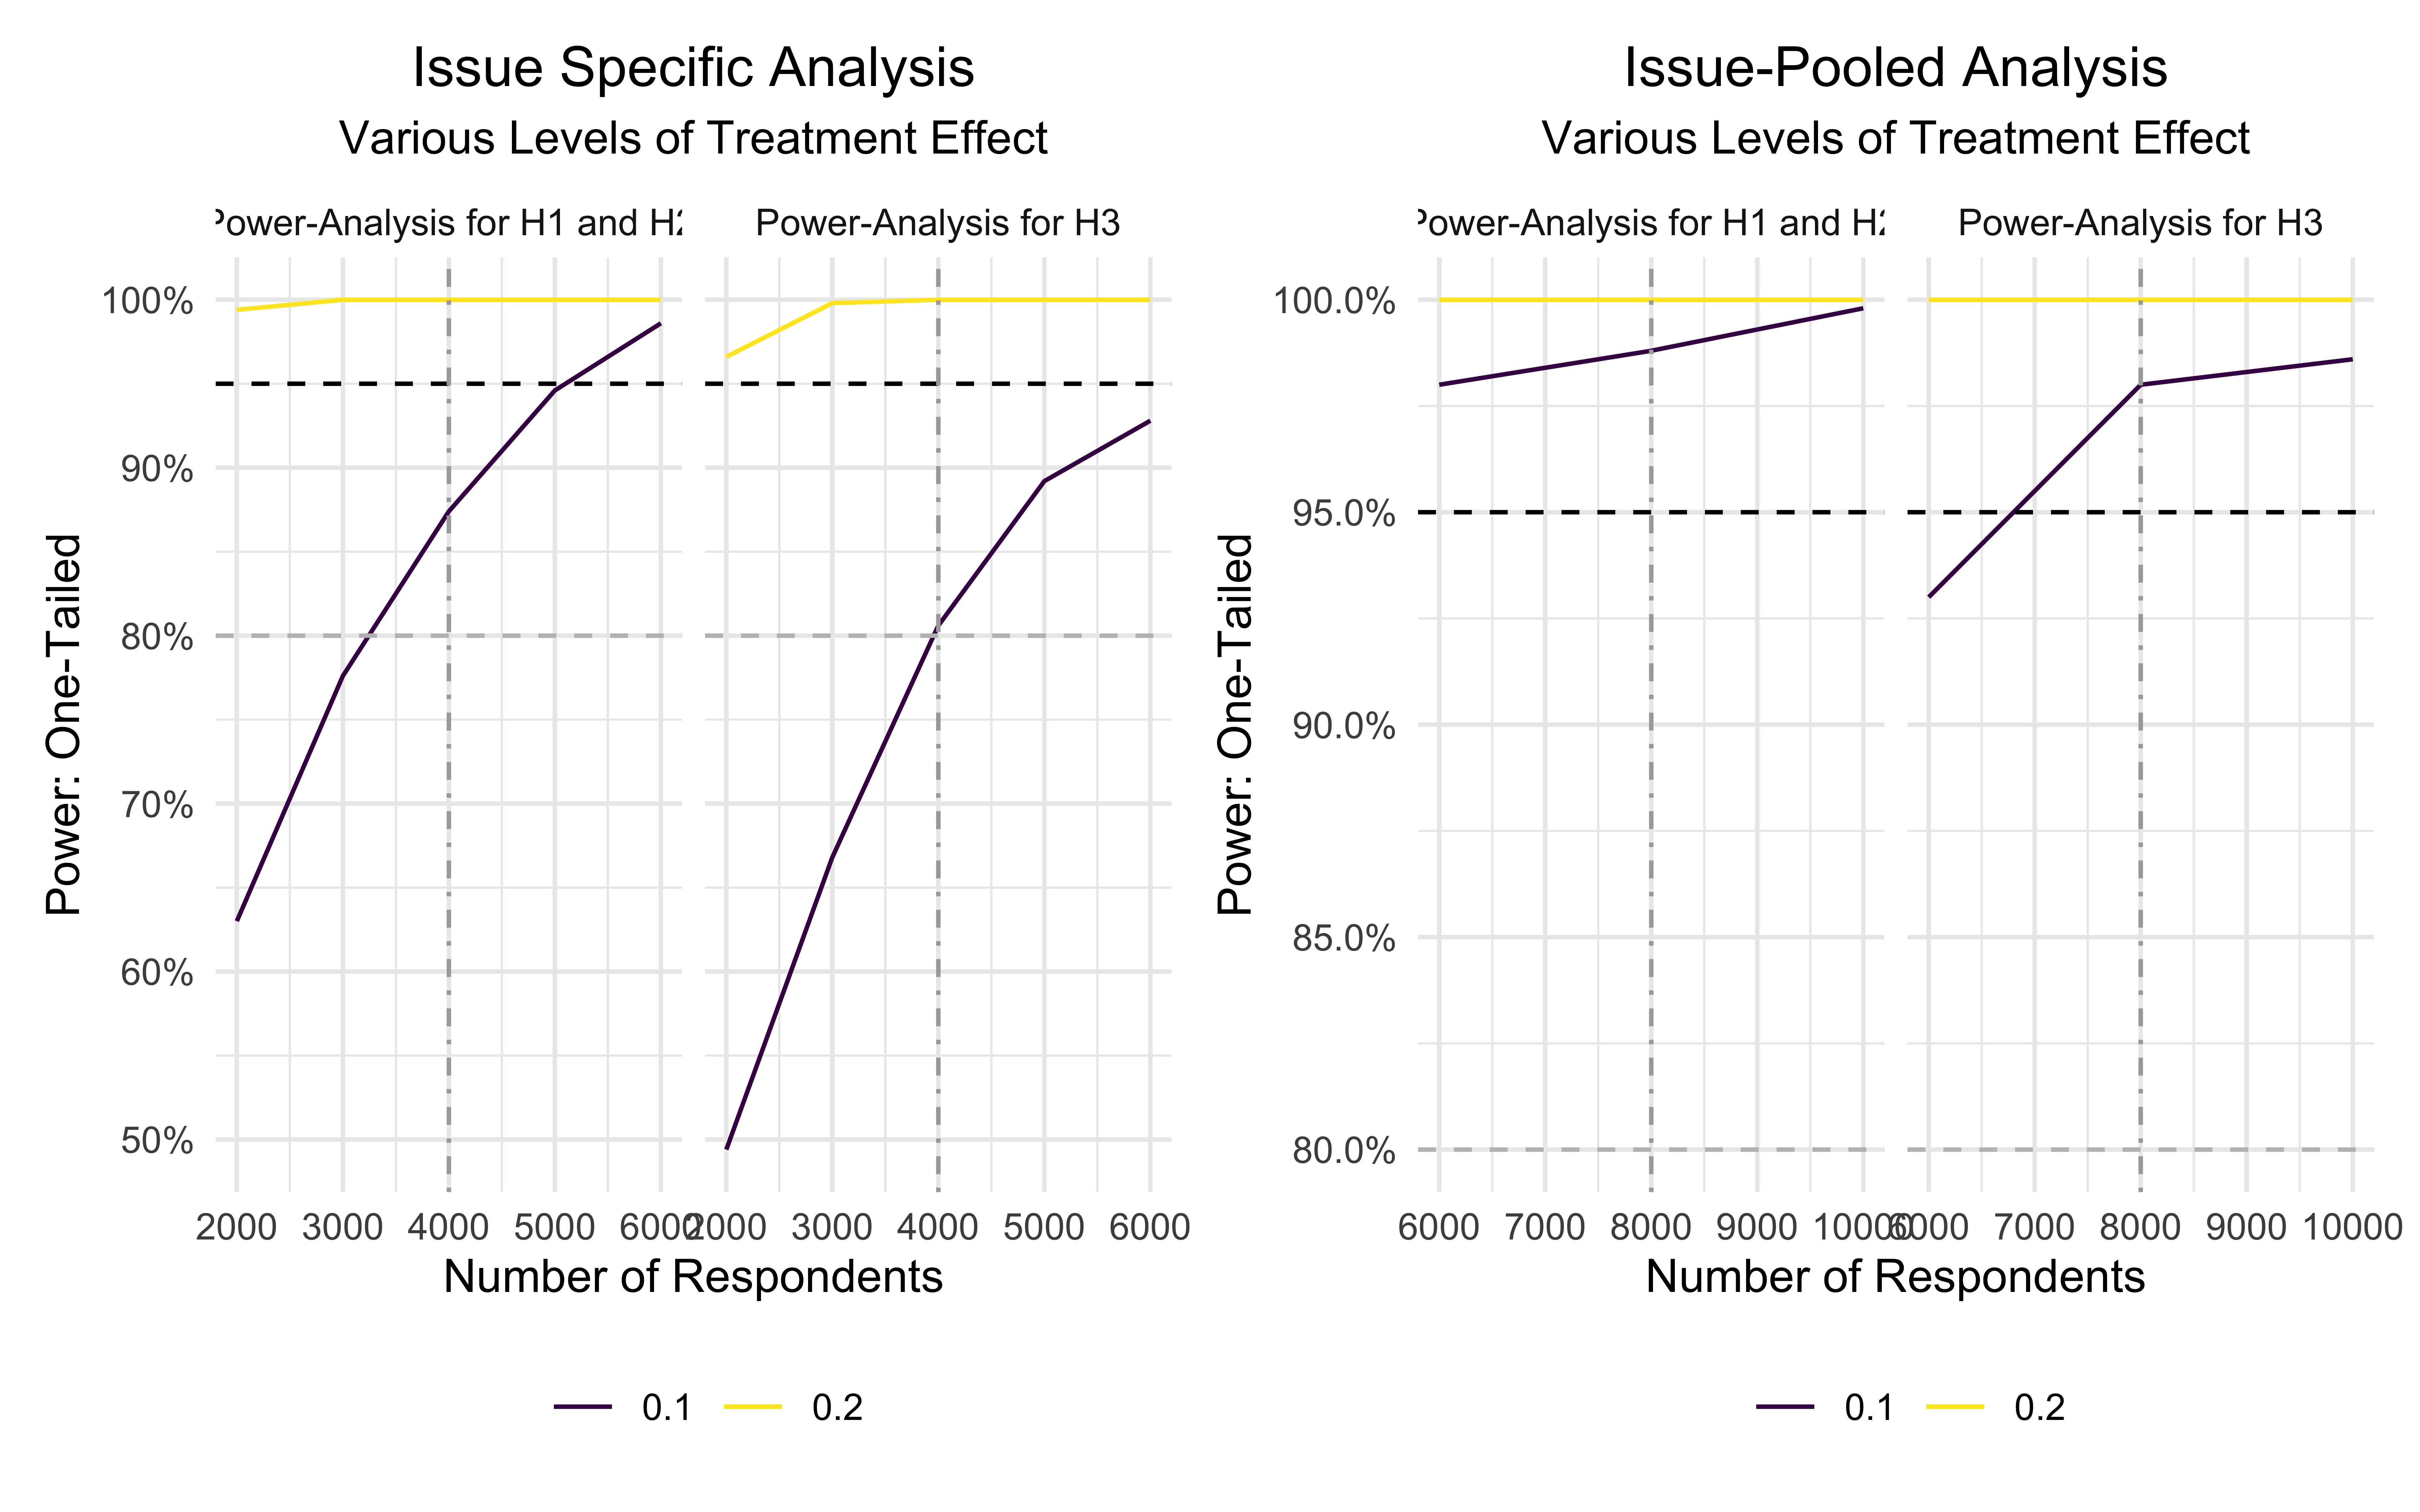
\includegraphics[width=1\linewidth]{/Users/marikenvandervelden/Dropbox/Papers/veni_project_mm/willingness-to-accept-compromises/docs/pre-analysis-plan/power_analysis-pooled} 

}

\caption{\label{fig:power1}Power Analysis}\label{fig:power}
\end{figure}

\hypertarget{measures}{%
\section{Measures}\label{measures}}

\hypertarget{dependent-variables}{%
\subsection{Dependent Variables}\label{dependent-variables}}

We rely on three measures reflecting different aspects of how people
evaluate parties as trustworthy. Measure 1 is used to test the
hypothesis, measure 2 and 3 are used exploratively.

\begin{enumerate}
\def\labelenumi{\arabic{enumi}.}
\item
  \emph{General trust} This measure exists of a statement on whether or
  not you trust a party -- see Table \ref{tab:dv} \texttt{DV1}. The
  statement is measured on a 10-point scale: From
  \texttt{do\ not\ trust\ at\ all} to \texttt{trust\ completely}.
\item
  \emph{Sincerity} In this measure respondents are asked to rank the
  party from very insincere (value of \texttt{0}) to very sincere (value
  of \texttt{10}) for the decision to (not) strike a compromise on the
  issue at stake. See Table \ref{tab:dv} \texttt{DV2} for the exact
  phrasing of the question.
\item
  \emph{Representation} In this measure, respondents are surveyed on how
  well the party is a good representative of the voters. The party can
  be evaluated on an 11-point scale from \texttt{very\ poorly} (value of
  \texttt{0}) till \texttt{very\ well} (value of 10). See Table
  \ref{tab:dv} \texttt{DV3} for the exact phrasing of the question.
\end{enumerate}

\begin{table}[!h]

\caption{\label{tab:dv}\label{tab:dv}Survey Questions - DV}
\centering
\begin{tabular}[t]{>{\raggedright\arraybackslash}p{3cm}>{\raggedright\arraybackslash}p{7cm}>{\raggedright\arraybackslash}p{7cm}}
\toprule
Variable & Wording ENG & Wording DE\\
\midrule
\cellcolor{gray!6}{trust (DV1)} & \cellcolor{gray!6}{Based on the Instagram post, to what extent do you trust [PARTY]} & \cellcolor{gray!6}{Der Instagram-Nachricht nach zu urteilen, wie sehr würden Sie [PARTY] vertrauen?}\\
sincere (DV2) & Based on the Instagram post, to what extent do you think [PARTY] is sincere? & Und inwieweit denken Sie, dass [PARTY] der Instagram-Nachricht nach aufrichtig gehandelt hat?\\
\cellcolor{gray!6}{representation (DV3)} & \cellcolor{gray!6}{Based on the Instagram post, to what extent do you think [PARTY] does a good job in representing its voters?} & \cellcolor{gray!6}{Und inwiefern denken Sie, dass [PARTY] ihre Wähler gut vertritt in Anbetracht der Instagram-Nachricht?}\\
\bottomrule
\end{tabular}
\end{table}

~

\hypertarget{control-variables}{%
\subsection{Control Variables}\label{control-variables}}

As control variables, the following \emph{demographics} are measured:
gender, age, education, geographical region, level of urbanness, vote
choice in the 2021 parliamentary elections, employment, and income. For
the analysis, only variables that are unbalanced over the experimental
conditions will be included. Table \ref{tab:demographics} gives an
overview of the questions asked in the survey as well as their English
translations.

\begin{itemize}
\item
  \emph{Gender} is measured as \texttt{sex} based on the advice of
  Kieskompas. The answer categories are \texttt{Male} (value of
  \texttt{1}), \texttt{Female} (value of \texttt{0}), and
  \texttt{No\ answer} (value of \texttt{999}).
\item
  \emph{Age} is measured using 6 categories: \texttt{17\ or\ younger},
  \texttt{18-\/-29}, \texttt{30-\/-39}, \texttt{40-\/-49},
  \texttt{50-\/-59}, \texttt{60-\/-74}.
\item
  \emph{Education} is measured as the highest successfully completed
  level of education, recoded into four categories: \texttt{low},
  \texttt{middle}, \texttt{high}, and \texttt{none}. I create dummy
  variables for each level of education with the lowest category as base
  category.
\item
  \emph{Urbanness} Respondents are asked for what the type of location
  they live: \texttt{big\ city}, \texttt{suburb\ of\ a\ large\ city},
  \texttt{middle-szed\ or\ small\ city}, \texttt{rural\ village},
  \texttt{detached\ house\ in\ the\ countryside},
  \texttt{don\textquotesingle{}t\ know/won\textquotesingle{}t\ say}.
\item
  \emph{Vote Recall} Respondents were asked which party they voted for
  in the last election with their second vote. Answering categories
  were: \texttt{CDU/CSU}, \texttt{SPD}, \texttt{AfD}, \texttt{FDP},
  \texttt{DIE\ LINKE}, \texttt{BÜNDNIS\ 90/DIE\ GRÜNEN},
  \texttt{Other\ party:},
  \texttt{I\ didn\textquotesingle{}t\ vote/wasn\textquotesingle{}t\ eligble\ to\ vote},
  \texttt{Don\textquotesingle{}t\ know/won\textquotesingle{}t\ say}.
\item
  \emph{Employment} Respondents were asked which category of employment
  -- \texttt{Full-time\ employed}, \texttt{Part-time\ employed},
  \texttt{Entrepreneur},
  \texttt{Unemployed\ and\ searching\ for\ a\ job},
  \texttt{Unemployed\ and\ not\ searching\ for\ a\ job\ or\ incapacitated},
  \texttt{Housewife/Househusband\ or\ else}, \texttt{Retired},
  \texttt{Student\ or\ full-time\ education} -- applied most to them.
\item
  \emph{Income} Respondents were questioned on their monthly income in
  bins of €500 -- \texttt{€500\ or\ less}, \texttt{€501-€1000},
  \texttt{€1001-€1500}, \texttt{€1501-€2000}, \texttt{€2001-€2500},
  \texttt{€2501-€3000}, \texttt{€3001-€3500}, \texttt{€3501-€4000},
  \texttt{€4501-€7500}, \texttt{€7501\ or\ more} -- as well as giving
  them the options of \texttt{won\textquotesingle{}t\ \ say} and
  \texttt{don\textquotesingle{}t\ know}.
\item
  \emph{Geographical region} is measured using the same questions as the
  \href{https://www.gesis.org/wahlen/gles}{German Longitudinal Election
  Study}, asking respondents where they are born and currently live,
  differentiating between the different German provinces
  (\emph{Bundesl\{"a\}nder}): Baden-W\{"u\}rtemberg, Bavaria, Berlin,
  Brandenburg, Bremen, Hamburg, Hessen, Lower Saxony,
  Mecklenburg-Western Pomerania, North Rhine- Westphalia,
  Rhineland-Palatinate, Saarland, Saxony, Saxony-Anholt,
  Schleswig-Holstein, and Thuringia.
\end{itemize}

\begin{table}[!h]

\caption{\label{tab:demographics}\label{tab:demographics}Survey Questions - Demographics}
\centering
\begin{tabular}[t]{>{\raggedright\arraybackslash}p{3cm}>{\raggedright\arraybackslash}p{7cm}>{\raggedright\arraybackslash}p{7cm}}
\toprule
Variable & Wording ENG & Wording DE\\
\midrule
\cellcolor{gray!6}{gender (D1)} & \cellcolor{gray!6}{Which gender do you feel you belong to?} & \cellcolor{gray!6}{Welchem Geschlecht fühlen Sie sich zugehörig?}\\
age (D2) & To which of the following age groups do you belong? & Zu welcher der nachfolgenden Altersgruppen gehören Sie?\\
\cellcolor{gray!6}{education (D3)} & \cellcolor{gray!6}{What is your highest educational qualification?} & \cellcolor{gray!6}{Was ist Ihr höchster Bildungsabschluss?}\\
geographical-region (D4) & Which of the following categories best describes where you live? & Welche der folgenden Kategorien beschreibt am besten, wo Sie wohnen?\\
\cellcolor{gray!6}{vote-recall2 (D6)} & \cellcolor{gray!6}{Which party did you vote for with your second vote in the last federal election in September 2021?} & \cellcolor{gray!6}{Welche Partei haben Sie bei der letzten Bundestagswahl im September 2021 mit Ihrer Zweitstimme gewählt?}\\
\addlinespace
employment (D7) & Now we would like to ask you something about your employment. Which of this list applies to you? & Nun möchten wir Sie gerne etwas zu Ihrer Erwerbstätigkeit fragen. Was von dieser Liste trifft auf Sie zu?\\
\cellcolor{gray!6}{income (D8)} & \cellcolor{gray!6}{What is the total monthly net income of your household? This refers to the sum that remains after deducting taxes and social security contributions.} & \cellcolor{gray!6}{Wie hoch ist das monatliche Netto-Einkommen Ihres Haushaltes insgesamt? Gemeint ist die Summe, die nach Abzug von Steuern und Sozialversicherungsbeiträgen übrig bleibt.}\\
living-place (D9) & In which federal state or on the territory of which present federal state do you currently live? & Im welchen Bundesland bzw. auf dem Gebiet welches heutigen Bundeslandes wohnen Sie derzeit?\\
\cellcolor{gray!6}{birth-place (D10)} & \cellcolor{gray!6}{And in which federal state or on the territory of which present federal state were you born?} & \cellcolor{gray!6}{Und in welchem Bundesland bzw. auf dem Gebiet welches heutigen Bundeslandes wurden Sie geboren?}\\
\bottomrule
\end{tabular}
\end{table}

In addition, pre-treatment, respondents' ideological position, position
on and salience of the issues speed limit, top tax, and Cannabis
legalization, political knowledge and interest are measured (see Tables
\ref{tab:pret1} and \ref{tab:pret2}). Those variables will only be
included in the analyses if balance checks indicate they are necessary.
Moreover, the variables will be used to explore heterogeneous
relationships.

\begin{itemize}
\item
  \emph{Ideological position} is measured using an 11-point scale
  ranging from left (\texttt{0}) to right (\texttt{10}).
\item
  \emph{Position on issues} is measured by forcing participants to
  choose whether or not the government should implement a policy:
  \texttt{implement\ speed\ limit}, \texttt{increase\ of\ top\ tax},
  \texttt{legalize\ cannabis}.
\item
  \emph{Salience of issues} is measured using an 11-point scale ranging
  from not at all important (\texttt{0}) to very important
  (\texttt{10}).
\end{itemize}

\begin{table}[!h]

\caption{\label{tab:pret}\label{tab:pret1}Survey Questions - PreTreatment Questions (1)}
\centering
\begin{tabular}[t]{>{\raggedright\arraybackslash}p{3cm}>{\raggedright\arraybackslash}p{7cm}>{\raggedright\arraybackslash}p{7cm}}
\toprule
Variable & Wording ENG & Wording DE\\
\midrule
\cellcolor{gray!6}{issue-pref-forced (PT1)} & \cellcolor{gray!6}{In your opinion, should the federal government implement the following policy proposals? Please select the response option that most closely matches your opinion.} & \cellcolor{gray!6}{Sollte die Bundesregierung Ihrer Meinung nach die folgenden politischen Vorschläge umsetzen? Bitte wählen Sie die Antwortoption, die Ihrer Meinung am ehesten entspricht.}\\
general speed limit (PT1-1) & General speed limit. & Generelles Tempolimit\\
\cellcolor{gray!6}{increase of top tax (PT1-2)} & \cellcolor{gray!6}{Increase the top tax rate} & \cellcolor{gray!6}{Erhöhung des Spitzensteuersatzes}\\
legalization of cannabis (PT1-3) & Cannabis Legalization. & Cannabis-Legalisierung\\
\cellcolor{gray!6}{issue-importance (PT3)} & \cellcolor{gray!6}{How important are the following issues to you?} & \cellcolor{gray!6}{Wie wichtig sind die folgenden Themen für Sie?}\\
\addlinespace
general speed limit (PT3-1) & General speed limit & Generelles Tempolimit\\
\cellcolor{gray!6}{increase of top tax (PT3-2)} & \cellcolor{gray!6}{Increasing the top tax rate} & \cellcolor{gray!6}{Erhöhung des Spitzensteuersatzes}\\
legalization of cannabis (PT3-3) & Cannabis legalization & Cannabis-Legalisierung\\
\cellcolor{gray!6}{political-knowledge1 (PT4)} & \cellcolor{gray!6}{In the federal election, you have two votes, a first vote and a second vote. How is that actually, which of the two votes is decisive for the distribution of seats in the Bundestag?} & \cellcolor{gray!6}{Bei der Bundestagswahl haben Sie ja zwei Stimmen, eine Erststimme und eine Zweitstimme. Wie ist das eigentlich, welche der beiden Stimmen ist ausschlaggebend für die Sitzverteilung im Bundestag?}\\
political-knowledge2 (PT5) & Now we would like to know from you, from what percentage of the second votes a party can send deputies in any case in the Bundestag? & Jetzt möchten wir gerne von Ihnen wissen, ab wie viel Prozent der Zweitstimmen eine Partei auf jeden Fall Abgeordnete in den Bundestag entsenden kann?\\
\addlinespace
\cellcolor{gray!6}{political-knowledge3 (PT6)} & \cellcolor{gray!6}{And can you say approximately what the current unemployment rate is in Germany? Is it lower or higher than 10 percent?} & \cellcolor{gray!6}{Und können Sie ungefähr sagen, wie hoch die derzeitige Arbeitslosenquote in Deutschland ist? Ist sie niedriger oder höher als 10 Prozent?}\\
\bottomrule
\end{tabular}
\end{table}

\begin{table}[!h]

\caption{\label{tab:pret}\label{tab:pret2}Survey Questions - PreTreatment Questions (2)}
\centering
\begin{tabular}[t]{>{\raggedright\arraybackslash}p{3cm}>{\raggedright\arraybackslash}p{7cm}>{\raggedright\arraybackslash}p{7cm}}
\toprule
Variable & Wording ENG & Wording DE\\
\midrule
\cellcolor{gray!6}{political-interest (PT7)} & \cellcolor{gray!6}{Once speaking in general terms: How interested are you in politics - very strongly, strongly, moderately, less strongly, or not at all?} & \cellcolor{gray!6}{Einmal ganz allgemein gesprochen: Wie stark interessieren Sie sich für Politik – sehr stark, stark, mittelmäßig, weniger stark oder überhaupt nicht?}\\
RILE (PT8) & In politics, people often talk about 'left' and 'right.' Where would you classify yourself? & In der Politik reden die Leute häufig von 'links' und 'rechts'. Wo würden Sie sich selbst einordnen?\\
\cellcolor{gray!6}{in-party (S1)} & \cellcolor{gray!6}{If you had to choose, which of the following parties would you be most likely to vote for in the next federal election?} & \cellcolor{gray!6}{Wenn Sie sich entscheiden müssten, welche der folgenden Parteien würden Sie bei der nächsten Bundestagswahl am ehesten wählen?}\\
in-party-strength (S2) & How strongly or how weakly do you identify with this party: very strongly, fairly strongly, moderately, fairly weakly, or very weakly? & Wie stark oder wie schwach indentifizieren Sie sich mit dieser Partei: sehr stark, ziemlich stark, mäßig, ziemlich schwach, oder sehr schwach?\\
\bottomrule
\end{tabular}
\end{table}

\begin{itemize}
\item
  \emph{Political knowledge} is measured with three items. First,
  respondents are asked which of the two votes is determinative for the
  seat distribution in parliament: \texttt{first\ vote},
  \texttt{second\ vote}, \texttt{both},
  \texttt{don\textquotesingle{}t\ know}. Secondly, respondents are asked
  about the electoral threshold. Last, respondents are asked whether or
  not the unemployment rate is over ten procent.
\item
  \emph{Political interest} is measured by asking people how strongly
  they are interested in politics using a 5-point Likert-scale
  (\texttt{very\ strong}, \texttt{strong}, \texttt{medium},
  \texttt{less\ strong}, \texttt{not\ at\ all}) and a
  \texttt{don\textquotesingle{}t\ know/won\textquotesingle{}t\ say}
  option.
\item
  \emph{In-party} is measured by forcing people to choose beween the
  four parties of the experiment (\texttt{CDU}, \texttt{die\ Grünen},
  \texttt{FDP}, and \texttt{SPD}) to determine which treatment they will
  be shown.
\item
  \emph{In-party strength} is measured by asking people how strongly
  they identify with the party uing a 5-point Likert-scale:
  \texttt{very\ strong}, \texttt{strong}, \texttt{medium},
  \texttt{less\ strong}, \texttt{not\ at\ all}
\end{itemize}

\hypertarget{attention-checks}{%
\subsection{Attention Checks}\label{attention-checks}}

We include two attention checks in the survey. The first one is after
the demographic covariates, the second one is asked just before
respondents enter the round of the experimental treatments. The
attention checks are taken from Berinsky, Margolis, and Sances (2014)
and adapted to the German context by the authors. If a respondents fails
the first attention check, a warning appears and the respondent can only
continue with the survey once the respondent has correctly answered the
question correctly. The second attention check also has a warning --
meaning that respondents have to select two options -- but if they fail
to correctly pass the check, they are excluded. Each excluded respondent
due to failing an attention check is replaced with another ``good
respondent".

\textbf{Attention Check 1} When a big news story breaks people often go
online to get up-to-the-minute details on what is going on. We want to
know which websites people trust to get this information. We also want
to know if people are paying attention to the question. To show that you
have read this much, please ignore the question and select BILD-Zeitung
and Süddeutsche Zeitung as your two answers. When there is a big news
story, which is the one news website you would visit first? (Please only
choose one). Eight (German) news outlets are provided to choose from.
Respondents pass the attention check if they select \emph{BILD-Zeitung}
and \emph{Süddeutsche Zeitung}.

\textbf{Attention Check 2}: We would like to get a sense of your general
preferences. Most modern theories of decision making recognize that
decisions do not take place in a vacuum. Individual preferences and
knowledge, along with situational variables can greatly impact the
decision process. To demonstrate that you've read this much, just go
ahead and select both red and green among the alternatives below, no
matter what your favourite color is. Yes, ignore the question below and
select both of those options. What is your favourite color? Six colors
are provided to choose from, respondents pass the attention check if
they select red and green.

\hypertarget{post-treatment-variables}{%
\subsection{Post-Treatment Variables}\label{post-treatment-variables}}

Post-treatment, the heterogeneous treatments (H4 and H5), manipulation
checks, cultural position, and populist attitudes are surveyed.

\begin{itemize}
\item
  \emph{Principledness} This is measured in two different ways. First,
  following Arceneaux (2019), , we measure principledness with using the
  Ethical Positions Questionnaire using a 7-point Likert scale
  (\texttt{Strongly\ Disagree}, \texttt{Disagree},
  \texttt{Somewhat\ Disagree}, \texttt{Neither\ Agree\ nor\ Disagree},
  \texttt{Somewhat\ Agree}, \texttt{Agree}, \texttt{Strongly\ Agre}). We
  reduce the initial 20 statements to 12 based on this
  \href{https://github.com/MarikenvdVelden/willingness-to-accept-compromises/blob/main/docs/pre-analysis-plan/absolutism_irt.pdf}{analysis},
  where statements 1--6 measure idealism and statements 7-- 12 measure
  relativism; absolutism is the combination of idealism with the
  rejection of relativism. If \texttt{Cronbach\textquotesingle{}s}
  \(\alpha\) \texttt{=\textgreater{}0.8}, we will construct an additive
  scale for this measure.When \texttt{Cronbach\textquotesingle{}s}
  \(\alpha\) \texttt{\textless{}0.8}, we will add the statement as
  seperate dependent variables in the multiverse analysis. Secondly, we
  use Ryan (2017)'s measure of Willingness to Accept (WtA) Benefits,
  where participants imagine to receive money (\texteuro \texttt{0},
  \texteuro \texttt{1}, \texteuro \texttt{2}, \texteuro \texttt{3},
  \texteuro \texttt{4}) but donate the same amount of money to an
  organization that is against their preferred policy position.
\item
  \emph{Mutual trust} is measured using three items from the European
  Social Survey using an 11-point scale, where \texttt{0} is the most
  negative answer, and \texttt{10} the most positive one. Respondents
  are asked whether they think most people can be trusted, most people
  try to take advantage of you, and most people are willing to help
  others. If \texttt{Cronbach\textquotesingle{}s} \(\alpha\)
  \texttt{=\textgreater{}0.8}, we will construct an additive scale for
  this measure. When \texttt{Cronbach\textquotesingle{}s} \(\alpha\)
  \texttt{\textless{}0.8}, we will add the statement as seperate
  dependent variables in the multiverse analysis.
\item
  \emph{Cultural position} is measured by asking if people find it
  important if people are born in Germany, have German ancestors, are
  able to speak German, and conform to the German norms and values using
  a 5-point Likert-scale (\texttt{Very\ importnat}, \texttt{Important},
  \texttt{Neutral}, \texttt{Unimportant}, \texttt{Very\ unimportant}).
\item
  \emph{Populism attitudes} We measure populist attitudes with the scale
  developed by Akkerman, Mudde, and Zaslove (2014) with a 5-point
  Likert-scale ranging (\texttt{Very\ much\ disagree},
  \texttt{Disagree}, \texttt{Neutral}, \texttt{Agree},
  \texttt{Very\ much\ agree}). For the statements, see Table XX.
\end{itemize}

\begin{table}[!h]

\caption{\label{tab:post}\label{tab:post1}Survey Questions - PostTreatment Questions (1)}
\centering
\begin{tabular}[t]{>{\raggedright\arraybackslash}p{3cm}>{\raggedright\arraybackslash}p{7cm}>{\raggedright\arraybackslash}p{7cm}}
\toprule
Variable & Wording ENG & Wording DE\\
\midrule
\cellcolor{gray!6}{princpledness2 (HT1a)} & \cellcolor{gray!6}{Below you will find a selection of general statements. We are interested in the extent to which you agree or disagree with the individual statements.} & \cellcolor{gray!6}{Im Folgenden finden Sie eine Auswahl an allgemeinen Aussagen. Uns interessiert, inwieweit Sie den einzelnen Aussagen zustimmen oder nicht zustimmen.}\\
princpledness2 (HT1a-1) & A person should be careful that their actions never intentionally cause harm to another person, even in a small way. & Eine Person sollte darauf achten, dass ihre Handlungen niemals absichtlich einen anderen Menschen Schaden zufügen, auch nicht in geringem Maße.\\
\cellcolor{gray!6}{princpledness2 (HT1a-2)} & \cellcolor{gray!6}{Putting others at risk should never be tolerated, no matter how small the risks.} & \cellcolor{gray!6}{Die Gefährdung anderer sollte niemals toleriert werden, unabhängig davon, wie gering die Risiken auch sein mögen.}\\
princpledness2 (HT1a-3) & The occurrence of potential harm to others is always wrong, regardless of the benefits. & Das Eintreten eines potenziellen Schadens für andere ist immer falsch, unabhängig von den Vorteilen, die sich daraus ergeben.\\
\cellcolor{gray!6}{princpledness2 (HT1a-4)} & \cellcolor{gray!6}{One should never hurt another person psychologically or physically.} & \cellcolor{gray!6}{Man sollte eine andere Person niemals psychisch oder physisch verletzen.}\\
\addlinespace
princpledness2 (HT1a-5) & One should not take any action that could in any way threaten the dignity and well-being of another person. & Man sollte keine Handlung vornehmen, die in irgendeiner Weise die Würde und das Wohlbefinden eines anderen Menschen bedrohen könnte.\\
\cellcolor{gray!6}{princpledness2 (HT1a-6)} & \cellcolor{gray!6}{If an act could harm an innocent third party, it should not be done.} & \cellcolor{gray!6}{Wenn eine Handlung einem unschuldigen Dritten schaden könnte, sollte sie nicht vorgenommen werden.}\\
princpledness2b (HT1b) & Im Folgenden finden Sie eine Auswahl an allgemeinen Aussagen. Uns interessiert, inwieweit Sie den einzelnen Aussagen zustimmen oder nicht zustimmen. & Im Folgenden finden Sie eine Auswahl an allgemeinen Aussagen. Uns interessiert, inwieweit Sie den einzelnen Aussagen zustimmen oder nicht zustimmen.\\
\cellcolor{gray!6}{princpledness2 (HT1b-1)} & \cellcolor{gray!6}{There are no ethical principles that are so important that everyone must follow them.} & \cellcolor{gray!6}{Es gibt keine ethischen Grundsätze, die so wichtig sind, dass jeder sie befolgen muss.}\\
princpledness2 (HT1b-2) & What is ethical varies from situation to situation and from society to society. & Was ethisch ist, variiert von Situation zu Situation und von Gesellschaft zu Gesellschaft.\\
\bottomrule
\end{tabular}
\end{table}

\begin{table}[!h]

\caption{\label{tab:post}\label{tab:post2}Survey Questions - PostTreatment Questions (2)}
\centering
\begin{tabular}[t]{>{\raggedright\arraybackslash}p{3cm}>{\raggedright\arraybackslash}p{7cm}>{\raggedright\arraybackslash}p{7cm}}
\toprule
Variable & Wording ENG & Wording DE\\
\midrule
\cellcolor{gray!6}{princpledness2 (HT1b-3)} & \cellcolor{gray!6}{You cannot say that a certain kind of morality is more correct than another.} & \cellcolor{gray!6}{Man kann nicht sagen, dass eine bestimmte Art von Moral richtiger ist als eine andere.}\\
princpledness2 (HT1b-4) & The question of what is ethical for all can never be settled, for what is moral or immoral should be left to the individual. & Die Frage, was für alle ethisch ist, kann nie geklärt werden, denn was moralisch oder unmoralisch ist, sollte dem Einzelnen überlassen werden.\\
\cellcolor{gray!6}{princpledness2 (HT1b-5)} & \cellcolor{gray!6}{Moral values are simply personal rules that indicate how a person should behave and should not be used to judge others.} & \cellcolor{gray!6}{Moralische Werte sind einfach persönliche Regeln, die angeben, wie sich eine Person verhalten sollte, und sollten nicht dazu dienen, über andere zu urteilen.}\\
princpledness2 (HT1b-6) & Whether something is considered moral or immoral depends on the circumstances. & Ob etwas als moralisch oder unmoralisch eingestuft wird, hängt von den Umständen ab.\\
\cellcolor{gray!6}{princpledness1 (HT2)} & \cellcolor{gray!6}{Imagine being able to choose an amount from the list below, and the amount you choose will be credited to your account. The catch is that the amount you choose will also be donated to an association that vehemently for/against the introduction of a top tax/ speed limit. What amount would you choose?} & \cellcolor{gray!6}{Stellen Sie sich vor, Sie können einen Betrag aus der unten stehenden Liste auswählen, und der von Ihnen gewählte Betrag wird Ihrem Konto gutgeschrieben. Der Haken an der Sache ist, dass der von Ihnen gewählte Betrag auch an einen Verband gespendet wird, der sich vehement gegen/für die Einführung eines Spitzensteuersatzes/Generellen Tempolimits einsetzt. Welchen Betrag würden Sie auswählen?}\\
\addlinespace
mutual-trust1 (HT3a) & Do you think that most people can be trusted, or that you can't be careful enough when dealing with other people? Please tell us using this scale from 0 to 10. 0 means that you can't be careful enough, and 10 means that you can trust most people. & Glauben Sie, dass man den meisten Menschen vertrauen kann, oder dass man im Umgang mit anderen Menschen nicht vorsichtig genug sein kann? Bitte sagen Sie es uns anhand dieser Skala von 0 bis 10. 0 bedeutet, dass man nicht vorsichtig genug sein kann, und 10 bedeutet, dass man den meisten Menschen vertrauen kann.\\
\cellcolor{gray!6}{mutual-trust2 (HT3b)} & \cellcolor{gray!6}{Do you think most people try to take advantage of you when they have the opportunity, or do most people try to be fair?} & \cellcolor{gray!6}{Glauben Sie, dass die meisten Menschen versuchen, Sie auszunutzen, wenn sie die Gelegenheit dazu haben, oder versuchen die meisten Menschen, sich fair zu verhalten?}\\
mutual-trust3 (HT3c) & And do you think that people are mostly trying to be helpful, or that people are mostly looking out for their own advantage? & Und glauben Sie, dass die Menschen meistens versuchen, hilfsbereit zu sein, oder dass die Menschen meistens auf den eigenen Vorteil bedacht sind?\\
\cellcolor{gray!6}{cultural-position (HT4)} & \cellcolor{gray!6}{Some people think that the following points are important to be truly German. Others do not think they are important. How important do you think the following points are to being German?} & \cellcolor{gray!6}{Manche Leute meinen, dass die folgenden Punkte wichtig sind, um wirklich deutsch zu sein. Andere halten diese nicht für wichtig. Für wie wichtig halten Sie die folgenden Punkte, um deutsch zu sein?}\\
cultural-position (HT4-1) & To be born in Germany & in Deutschland geboren sein\\
\bottomrule
\end{tabular}
\end{table}

\begin{table}[!h]

\caption{\label{tab:post}\label{tab:post3}Survey Questions - PostTreatment Questions (3)}
\centering
\begin{tabular}[t]{>{\raggedright\arraybackslash}p{3cm}>{\raggedright\arraybackslash}p{7cm}>{\raggedright\arraybackslash}p{7cm}}
\toprule
Variable & Wording ENG & Wording DE\\
\midrule
\cellcolor{gray!6}{cultural-position (HT4-2)} & \cellcolor{gray!6}{to have German ancestors} & \cellcolor{gray!6}{deutsche Vorfahren haben}\\
cultural-position (HT4-3) & to be able to speak German & deutsch sprechen können\\
\cellcolor{gray!6}{cultural-position (HT4-4)} & \cellcolor{gray!6}{to adhere to German traditions and customs} & \cellcolor{gray!6}{sich an deutsche Traditionen und Gepflogenheiten halten}\\
populist-attitudes (POST1) & Now we would like to know your opinion on some general statements about politics. For each of the following statements, please indicate the extent to which you agree or disagree with it. & Jetzt möchten wir gerne Ihre Meinung zu einigen allgemeinen Aussagen zur Politik wissen. Bitte geben Sie zu jeder der folgenden Aussagen an, inwieweit Sie dieser zustimmen oder diese ablehnen.\\
\cellcolor{gray!6}{populist-attitudes (POST1-1)} & \cellcolor{gray!6}{What is called compromise in politics is really just a betrayal of principles.} & \cellcolor{gray!6}{Was in der Politik Kompromiss genannt wird, ist in Wirklichkeit nur ein Verrat von Prinzipien.}\\
\addlinespace
populist-attitudes (POST1-2) & Citizens, not politicians, should make the most important policy decisions. & Die Bürger, und nicht die Politiker, sollten die wichtigsten politischen Entscheidungen treffen.\\
\cellcolor{gray!6}{populist-attitudes (POST1-3)} & \cellcolor{gray!6}{The members of the German Bundestag must follow the will of the citizens.} & \cellcolor{gray!6}{Die Abgeordneten des Deutschen Bundestags müssen dem Willen der Bürger Folge leisten.}\\
populist-attitudes (POST1-4) & The political differences between elites and citizens are greater than the differences between citizens. & Die politischen Unterschiede zwischen den Eliten und den Bürgern sind größer als die Unterschiede zwischen Bürgern.\\
\cellcolor{gray!6}{populist-attitudes (POST1-5)} & \cellcolor{gray!6}{Elected officials talk too much and take too little action} & \cellcolor{gray!6}{Die Politiker reden zu viel und machen zu wenig.}\\
populist-attitudes (POST1-6) & A citizen would better represent my interests than a professional politician. & Ein Bürger würde besser meine Interessen vertreten als ein Berufspolitiker.\\
\bottomrule
\end{tabular}
\end{table}

\begin{table}[!h]

\caption{\label{tab:post}\label{tab:post4}Survey Questions - PostTreatment Questions (4)}
\centering
\begin{tabular}[t]{>{\raggedright\arraybackslash}p{3cm}>{\raggedright\arraybackslash}p{7cm}>{\raggedright\arraybackslash}p{7cm}}
\toprule
Variable & Wording ENG & Wording DE\\
\midrule
\cellcolor{gray!6}{populist-attitudes (POST1-7)} & \cellcolor{gray!6}{In a democracy, it is important to compromise between different points of view.} & \cellcolor{gray!6}{In einer Demokratie ist es wichtig, Kompromisse zwischen unterschiedlichen Standpunkten zu schließen.}\\
populist-attitudes (POST1-8) & It is important to listen to the opinions of other groups. & Es ist wichtig, die Meinung anderer Gruppen anzuhören.\\
\cellcolor{gray!6}{manipulation-check1 (MC1)} & \cellcolor{gray!6}{Can you please tell us if [PARTY] would compromise(s) according to the Instagram message?} & \cellcolor{gray!6}{Können Sie uns bitte sagen, ob [PARTY] der Instagram-Nachricht zufolge einen Kompromiss eingehen würde(n)?}\\
manipulation-check2 (MC2) & Can you please tell us if the two parties have agreed to start coalition talks according to the Instagram message? & Können Sie uns bitte sagen, ob die beide Parteien der Instagram-Nachricht zufolge sich geinigt haben, Koalitionsverhandlungen aufzunehmen?\\
\cellcolor{gray!6}{reality-check (MC3)} & \cellcolor{gray!6}{The Instagram message you just saw represented a fictional scenario of coalition talks. Do you know which parties are currently holding exploratory talks in reality? Please select all applicable parties.} & \cellcolor{gray!6}{Die Instagram-Nachricht, die Sie gerade gesehen haben, stellte ein fiktives Szenario der Koalitionsverhandlungen dar. Wissen Sie, welche Parteien derzeit in der Wirklichkeit Sondierungsgespräche führen? Bitte wählen Sie alle zutreffenden Parteien aus.}\\
\bottomrule
\end{tabular}
\end{table}

\begin{itemize}
\tightlist
\item
  \emph{Manipulation checks}
\end{itemize}

\hypertarget{exclusion-criteria}{%
\subsection{Exclusion Criteria}\label{exclusion-criteria}}

Participants are required to respond to each question. Participants who
fail the second attention check will be excluded but replaced by another
participant.

\hypertarget{analysis}{%
\section{Analysis}\label{analysis}}

We test the hypotheses formulated in
\protect\hyperlink{expectations}{Section 1} by fitting linear
multivariate regressions separately for the two issues. In each model,
we will estimate the coefficient for whether the party compromised or
remained steadfast (H1), whether or not the coalition talks continued
(H2), and the interaction of compromise and the outcome (H3). We will
only add control variables in the analyses that are unbalanced, as
explained in \protect\hyperlink{balance-checks}{Section 4.1}.

\hypertarget{balance-checks}{%
\subsection{Balance Checks}\label{balance-checks}}

We will conduct a balance test based on demographics (age, gender,
education, geographical region, level of urbanness,employment, and
income), vote choice in the 2021 parliamentary elections, ideological
self-placement, political knowledge, political interest, party identity
strength, and positions on and salience of the three issues, using the
\texttt{cobalt} R package (Greifer 2021). If the groups are unbalanced
on one of these variables -- i.e.~standardized mean differences
\texttt{\textless{}0.05} -- I will add the covariates to the analyses. I
will use the code below to conduct the balance tests (see
\href{https://github.com/MarikenvdVelden/compromise-punish/tree/main/src/analysis/balance-test.R}{here}
for the R script).

\begin{Shaded}
\begin{Highlighting}[]
\NormalTok{covs <-}\StringTok{ }\NormalTok{d }\OperatorTok
\StringTok{  }\KeywordTok{mutate}\NormalTok{(}\DataTypeTok{treatment =} \KeywordTok{paste}\NormalTok{(compromise, outcome, }\DataTypeTok{sep =} \StringTok{"-"}\NormalTok{)) }\OperatorTok
\StringTok{  }\KeywordTok{select}\NormalTok{(treatment, D1}\OperatorTok{:}\NormalTok{D10, PT1}\OperatorTok{:}\NormalTok{PT8, S2) }

\NormalTok{balanced <-}\KeywordTok{bal.tab}\NormalTok{(treatment }\OperatorTok{~}\StringTok{ }\KeywordTok{factor}\NormalTok{(D1) }\OperatorTok{+}\StringTok{ }\NormalTok{D2 }\OperatorTok{+}
\StringTok{                     }\KeywordTok{factor}\NormalTok{(D3) }\OperatorTok{+}\StringTok{ }\NormalTok{D4 }\OperatorTok{+}\StringTok{ }\NormalTok{D5 }\OperatorTok{+}\StringTok{ }
\StringTok{                     }\KeywordTok{factor}\NormalTok{(D6) }\OperatorTok{+}\StringTok{ }\NormalTok{D7 }\OperatorTok{+}\StringTok{ }\NormalTok{D8 }\OperatorTok{+}\StringTok{ }\NormalTok{D9 }\OperatorTok{+}
\StringTok{                     }\NormalTok{D10 }\OperatorTok{+}\StringTok{ }\NormalTok{PT1_}\DecValTok{1} \OperatorTok{+}\StringTok{ }\NormalTok{PT1_}\DecValTok{2} \OperatorTok{+}\StringTok{ }\NormalTok{PT1_}\DecValTok{3} \OperatorTok{+}
\StringTok{                     }\NormalTok{PT3_}\DecValTok{1} \OperatorTok{+}\StringTok{ }\NormalTok{PT3_}\DecValTok{2} \OperatorTok{+}\StringTok{ }\NormalTok{PT3_}\DecValTok{3} \OperatorTok{+}\StringTok{ }\NormalTok{PT4 }\OperatorTok{+}\StringTok{ }
\StringTok{                     }\NormalTok{PT5 }\OperatorTok{+}\StringTok{ }\NormalTok{PT6 }\OperatorTok{+}\StringTok{ }\NormalTok{PT7 }\OperatorTok{+}\StringTok{ }\NormalTok{PT8 }\OperatorTok{+}\StringTok{ }\NormalTok{S2}
                     \KeywordTok{factor}\NormalTok{(F1) }\OperatorTok{+}\StringTok{ }\NormalTok{F2 }\OperatorTok{+}\StringTok{ }\KeywordTok{factor}\NormalTok{(F9),}
                     \DataTypeTok{data =}\NormalTok{ covs,}
          \DataTypeTok{thresholds =} \KeywordTok{c}\NormalTok{(}\DataTypeTok{m =} \FloatTok{0.05}\NormalTok{))[[}\DecValTok{1}\NormalTok{]] }
\end{Highlighting}
\end{Shaded}

\hypertarget{hypothesis-1}{%
\subsection{Hypothesis 1}\label{hypothesis-1}}

We test the \emph{steadfast hypothesis} using Equation \ref{eq:h1} and
the code chunk below. The coefficient of \(\beta_{1}\) denotes the
difference in the evaluation of steadfast and compromising parties If
the effect of \(\beta_{1}\) is positive and statistically significant,
the \textit{steadfast hypothesis} will be confirmed.

\begin{equation}\label{eq:h1}
  \begin{aligned}
    \hat{Y}_{Party \ Evaluation} = \beta_{0} + \beta_{1}Steadfast  +
    \beta_{2}Outcome + \beta_{4}Party\ ID + 
    \beta_{5}Party \ ID \ Strength + \nonumber \\
    \beta_{5}Unbalanced \ Covariates + \varepsilon
  \end{aligned}
\end{equation}

\begin{Shaded}
\begin{Highlighting}[]
\KeywordTok{source}\NormalTok{(here}\OperatorTok{::}\KeywordTok{here}\NormalTok{(}\StringTok{"src/lib/functions.R"}\NormalTok{))}

\NormalTok{df <-}\StringTok{ }\NormalTok{d }\OperatorTok\StringTok{ }
\StringTok{  }\KeywordTok{mutate}\NormalTok{(steadfast }\OperatorTok{==}\StringTok{ }\KeywordTok{if_else}\NormalTok{(compromise}\OperatorTok{==}\StringTok{"yes"}\NormalTok{, }\DecValTok{0}\NormalTok{, }\DecValTok{1}\NormalTok{)) }\OperatorTok
\StringTok{  }\KeywordTok{filter}\NormalTok{(issue }\OperatorTok{==}\StringTok{ "SpeedLimit"}\NormalTok{) }\OperatorTok
\StringTok{  }\KeywordTok{select}\NormalTok{(DV1, outcome, steadfast, S1, S2) }\OperatorTok
\NormalTok{h1_}\DecValTok{1}\NormalTok{ <-}\StringTok{ }\KeywordTok{lm}\NormalTok{(DV1 }\OperatorTok{~}\StringTok{  }\NormalTok{steadfast }\OperatorTok{+}\StringTok{ }\NormalTok{outcome }\OperatorTok{+}\StringTok{ }\KeywordTok{factor}\NormalTok{(S1) }\OperatorTok{+}\StringTok{ }\NormalTok{S2,}
                   \DataTypeTok{data =}\NormalTok{ df)}

\NormalTok{df <-}\StringTok{ }\NormalTok{d }\OperatorTok\StringTok{ }
\StringTok{  }\KeywordTok{mutate}\NormalTok{(steadfast }\OperatorTok{==}\StringTok{ }\KeywordTok{if_else}\NormalTok{(compromise}\OperatorTok{==}\StringTok{"yes"}\NormalTok{, }\DecValTok{0}\NormalTok{, }\DecValTok{1}\NormalTok{)) }\OperatorTok
\StringTok{  }\KeywordTok{filter}\NormalTok{(issue }\OperatorTok{==}\StringTok{ "TopTax"}\NormalTok{) }\OperatorTok
\StringTok{  }\KeywordTok{select}\NormalTok{(DV1, outcome, steadfast, S1, S2) }\OperatorTok
\NormalTok{h1_}\DecValTok{2}\NormalTok{ <-}\StringTok{ }\KeywordTok{lm}\NormalTok{(DV1 }\OperatorTok{~}\StringTok{  }\NormalTok{steadfast }\OperatorTok{+}\StringTok{ }\NormalTok{outcome }\OperatorTok{+}\StringTok{ }\KeywordTok{factor}\NormalTok{(S1) }\OperatorTok{+}\StringTok{ }\NormalTok{S2, }
                   \DataTypeTok{data =}\NormalTok{ df)}
\end{Highlighting}
\end{Shaded}

\hypertarget{hypothesis-2}{%
\subsection{Hypothesis 2}\label{hypothesis-2}}

We test the \emph{responsibility hypothesis} using Equation \ref{eq:h2}
and the code chunk below. The coefficient of \(\beta_{2}\) denotes the
difference in the evaluation of parties negotiating for coalition
government and those who stop talking to potential coalition partners.
If the effect of \(\beta_{2}\) is positive and statistically
significant, the \emph{responsibility hypothesis} will be confirmed.

\begin{equation}\label{eq:h2}
  \begin{aligned}
    \hat{Y}_{Party \ Evaluation} = \beta_{0} + \beta_{1}Compromise  +
    \beta_{2}Outcome + \beta_{3}Party \ ID + \nonumber \\
    \beta_{4}Party \ ID \ Strength +
    \beta_{5}Unbalanced \ Covariates + \varepsilon
  \end{aligned}
\end{equation}

\begin{Shaded}
\begin{Highlighting}[]
\KeywordTok{source}\NormalTok{(here}\OperatorTok{::}\KeywordTok{here}\NormalTok{(}\StringTok{"src/lib/functions.R"}\NormalTok{))}

\NormalTok{df <-}\StringTok{ }\NormalTok{d }\OperatorTok\StringTok{ }
\StringTok{  }\KeywordTok{mutate}\NormalTok{(steadfast }\OperatorTok{==}\StringTok{ }\KeywordTok{if_else}\NormalTok{(compromise}\OperatorTok{==}\StringTok{"yes"}\NormalTok{, }\DecValTok{1}\NormalTok{, }\DecValTok{0}\NormalTok{),}
         \DataTypeTok{negotiation =} \KeywordTok{if_else}\NormalTok{(outcome}\OperatorTok{==}\StringTok{"negotiation"}\NormalTok{, }\DecValTok{1}\NormalTok{, }\DecValTok{0}\NormalTok{)) }\OperatorTok
\StringTok{  }\KeywordTok{filter}\NormalTok{(issue }\OperatorTok{==}\StringTok{ "SpeedLimit"}\NormalTok{) }\OperatorTok
\StringTok{  }\KeywordTok{select}\NormalTok{(DV1, negotiation, compromise, S1, S2) }\OperatorTok
\NormalTok{h2_}\DecValTok{1}\NormalTok{ <-}\StringTok{ }\KeywordTok{lm}\NormalTok{(DV1 }\OperatorTok{~}\StringTok{  }\NormalTok{compromise }\OperatorTok{+}\StringTok{ }\NormalTok{negotiation }\OperatorTok{+}\StringTok{ }\KeywordTok{factor}\NormalTok{(S1) }\OperatorTok{+}\StringTok{ }\NormalTok{S2,}
                   \DataTypeTok{data =}\NormalTok{ df)}

\NormalTok{df <-}\StringTok{ }\NormalTok{d }\OperatorTok\StringTok{ }
\StringTok{  }\KeywordTok{mutate}\NormalTok{(steadfast }\OperatorTok{==}\StringTok{ }\KeywordTok{if_else}\NormalTok{(compromise}\OperatorTok{==}\StringTok{"yes"}\NormalTok{, }\DecValTok{1}\NormalTok{, }\DecValTok{0}\NormalTok{),}
         \DataTypeTok{negotiation =} \KeywordTok{if_else}\NormalTok{(outcome}\OperatorTok{==}\StringTok{"negotiation"}\NormalTok{, }\DecValTok{1}\NormalTok{, }\DecValTok{0}\NormalTok{)) }\OperatorTok
\StringTok{  }\KeywordTok{filter}\NormalTok{(issue }\OperatorTok{==}\StringTok{ "TopTax"}\NormalTok{) }\OperatorTok
\StringTok{  }\KeywordTok{select}\NormalTok{(DV1, negotiation, compromise, S1, S2) }\OperatorTok
\NormalTok{h2_}\DecValTok{2}\NormalTok{ <-}\StringTok{ }\KeywordTok{lm}\NormalTok{(DV1 }\OperatorTok{~}\StringTok{  }\NormalTok{compromise }\OperatorTok{+}\StringTok{ }\NormalTok{negotiation }\OperatorTok{+}\StringTok{ }\KeywordTok{factor}\NormalTok{(S1) }\OperatorTok{+}\StringTok{ }\NormalTok{S2,}
                   \DataTypeTok{data =}\NormalTok{ df)}
\end{Highlighting}
\end{Shaded}

\hypertarget{hypothesis-3}{%
\subsection{Hypothesis 3}\label{hypothesis-3}}

We test the \emph{compromise hypothesis} using Equation \ref{eq:h3} and
the code chunk below. The coefficient of \(\beta_{1}\) denotes the
difference in the evaluation of steadfast and compromising parties. The
coefficient of \(\beta_{2}\) denotes the difference in the evaluation of
parties negotiating for coalition government and those who stop talking
to potential coalition partners. The coefficient of \(\beta_{3}\) is the
interaction of the \(\beta_{1}\) and \(\beta_{2}\). If the Average
Marginal Effect of \(\beta_{1}\) is positive and statistically
significant when \(\beta_{2} = 1\) (i.e.~congruence), then H3 will be
confirmed.

\begin{equation}\label{eq:h3}
  \begin{aligned}
    \hat{Y}_{Party \ Evaluation} = \beta_{0} + \beta_{1}Compromise  + 
    \beta_{2}Outcome + \beta_{3}Compromise * Outcome + \nonumber \\
    \beta_{4}Party\ ID + \beta_{5}Party \ ID \ Strength + 
    \beta_{6}Unbalanced \ Covariates + \varepsilon
  \end{aligned}
\end{equation}

\begin{Shaded}
\begin{Highlighting}[]
\KeywordTok{source}\NormalTok{(here}\OperatorTok{::}\KeywordTok{here}\NormalTok{(}\StringTok{"src/lib/functions.R"}\NormalTok{))}

\NormalTok{df <-}\StringTok{ }\NormalTok{d }\OperatorTok\StringTok{ }
\StringTok{  }\KeywordTok{mutate}\NormalTok{(steadfast }\OperatorTok{==}\StringTok{ }\KeywordTok{if_else}\NormalTok{(compromise}\OperatorTok{==}\StringTok{"yes"}\NormalTok{, }\DecValTok{1}\NormalTok{, }\DecValTok{0}\NormalTok{),}
         \DataTypeTok{negotiation =} \KeywordTok{if_else}\NormalTok{(outcome}\OperatorTok{==}\StringTok{"negotiation"}\NormalTok{, }\DecValTok{1}\NormalTok{, }\DecValTok{0}\NormalTok{)) }\OperatorTok
\StringTok{  }\KeywordTok{filter}\NormalTok{(issue }\OperatorTok{==}\StringTok{ "SpeedLimit"}\NormalTok{) }\OperatorTok
\StringTok{  }\KeywordTok{select}\NormalTok{(DV1, negotiation, compromise, S1, S2) }\OperatorTok
\NormalTok{h3_}\DecValTok{1}\NormalTok{ <-}\StringTok{ }\KeywordTok{lm}\NormalTok{(DV1 }\OperatorTok{~}\StringTok{  }\NormalTok{compromise}\OperatorTok{*}\NormalTok{negotiation }\OperatorTok{+}\StringTok{ }\KeywordTok{factor}\NormalTok{(S1) }\OperatorTok{+}\StringTok{ }\NormalTok{S2,}
                   \DataTypeTok{data =}\NormalTok{ df)}

\NormalTok{df <-}\StringTok{ }\NormalTok{d }\OperatorTok\StringTok{ }
\StringTok{  }\KeywordTok{mutate}\NormalTok{(steadfast }\OperatorTok{==}\StringTok{ }\KeywordTok{if_else}\NormalTok{(compromise}\OperatorTok{==}\StringTok{"yes"}\NormalTok{, }\DecValTok{1}\NormalTok{, }\DecValTok{0}\NormalTok{),}
         \DataTypeTok{negotiation =} \KeywordTok{if_else}\NormalTok{(outcome}\OperatorTok{==}\StringTok{"negotiation"}\NormalTok{, }\DecValTok{1}\NormalTok{, }\DecValTok{0}\NormalTok{)) }\OperatorTok
\StringTok{  }\KeywordTok{filter}\NormalTok{(issue }\OperatorTok{==}\StringTok{ "TopTax"}\NormalTok{) }\OperatorTok
\StringTok{  }\KeywordTok{select}\NormalTok{(DV1, negotiation, compromise, S1, S2) }\OperatorTok
\NormalTok{h3_}\DecValTok{2}\NormalTok{ <-}\StringTok{ }\KeywordTok{lm}\NormalTok{(DV1 }\OperatorTok{~}\StringTok{  }\NormalTok{compromise}\OperatorTok{*}\NormalTok{negotiation }\OperatorTok{+}\StringTok{ }\KeywordTok{factor}\NormalTok{(S1) }\OperatorTok{+}\StringTok{ }\NormalTok{S2,}
                   \DataTypeTok{data =}\NormalTok{ df)}
\end{Highlighting}
\end{Shaded}

\hypertarget{hypothesis-4}{%
\subsection{Hypothesis 4}\label{hypothesis-4}}

We test the \emph{principled hypothesis} using Equation \ref{eq:h4} and
the code chunk below. The coefficient of \(\beta_{1}\) denotes the
difference in the evaluation of steadfast and compromising parties. The
coefficient of \(\beta_{3}\) denotes the difference in the evaluation of
parties for people with different levels of principledness. The
coefficient of \(\beta_{4}\) is the interaction of the \(\beta_{1}\) and
\(\beta_{3}\). When the Average Marginal Effect of \(\beta_{1}\) is
negative and statistically significant for higher values of
\(\beta_{3} = >\) (i.e.~principledness), H4 will be confirmed.

\begin{equation}\label{eq:h4}
  \begin{aligned}
      \hat{Y}_{Party \ Evaluation} = \beta_{0} + \beta_{1}Compromise  +
      \beta_{2}Outcome + \beta_{3}Principled  +\nonumber \\
      \beta_{4}Outcoume * Principled + 
      \beta_{5}Party\ ID + \beta_{6}Party \ ID \ Strength +\nonumber \\
      \beta_{5}Unbalanced \ Covariates + \varepsilon
    \end{aligned}
\end{equation}

\begin{Shaded}
\begin{Highlighting}[]
\KeywordTok{source}\NormalTok{(here}\OperatorTok{::}\KeywordTok{here}\NormalTok{(}\StringTok{"src/lib/functions.R"}\NormalTok{))}

\NormalTok{df <-}\StringTok{ }\NormalTok{d }\OperatorTok\StringTok{ }
\StringTok{  }\KeywordTok{mutate}\NormalTok{(steadfast }\OperatorTok{==}\StringTok{ }\KeywordTok{if_else}\NormalTok{(compromise}\OperatorTok{==}\StringTok{"yes"}\NormalTok{, }\DecValTok{1}\NormalTok{, }\DecValTok{0}\NormalTok{),}
         \DataTypeTok{negotiation =} \KeywordTok{if_else}\NormalTok{(outcome}\OperatorTok{==}\StringTok{"negotiation"}\NormalTok{, }\DecValTok{1}\NormalTok{, }\DecValTok{0}\NormalTok{)) }\OperatorTok
\StringTok{  }\KeywordTok{filter}\NormalTok{(issue }\OperatorTok{==}\StringTok{ "SpeedLimit"}\NormalTok{) }\OperatorTok
\StringTok{  }\KeywordTok{select}\NormalTok{(DV1, negotiation, compromise, HT1, S1, S2) }\OperatorTok
\NormalTok{h4_1a <-}\StringTok{ }\KeywordTok{lm}\NormalTok{(DV1 }\OperatorTok{~}\StringTok{  }\NormalTok{compromise }\OperatorTok{+}\StringTok{ }\NormalTok{negotiation}\OperatorTok{*}\NormalTok{HT1 }\OperatorTok{+}
\StringTok{                      }\KeywordTok{factor}\NormalTok{(S1) }\OperatorTok{+}\StringTok{ }\NormalTok{S2,}
                    \DataTypeTok{data =}\NormalTok{ df)}

\NormalTok{df <-}\StringTok{ }\NormalTok{d }\OperatorTok\StringTok{ }
\StringTok{  }\KeywordTok{mutate}\NormalTok{(steadfast }\OperatorTok{==}\StringTok{ }\KeywordTok{if_else}\NormalTok{(compromise}\OperatorTok{==}\StringTok{"yes"}\NormalTok{, }\DecValTok{1}\NormalTok{, }\DecValTok{0}\NormalTok{),}
         \DataTypeTok{negotiation =} \KeywordTok{if_else}\NormalTok{(outcome}\OperatorTok{==}\StringTok{"negotiation"}\NormalTok{, }\DecValTok{1}\NormalTok{, }\DecValTok{0}\NormalTok{)) }\OperatorTok
\StringTok{  }\KeywordTok{filter}\NormalTok{(issue }\OperatorTok{==}\StringTok{ "SpeedLimit"}\NormalTok{) }\OperatorTok
\StringTok{  }\KeywordTok{select}\NormalTok{(DV1, negotiation, compromise, HT2, S1, S2) }\OperatorTok
\NormalTok{h4_1b <-}\StringTok{ }\KeywordTok{lm}\NormalTok{(DV1 }\OperatorTok{~}\StringTok{  }\NormalTok{compromise }\OperatorTok{+}\StringTok{ }\NormalTok{negotiation}\OperatorTok{*}\NormalTok{HT2 }\OperatorTok{+}
\StringTok{                      }\KeywordTok{factor}\NormalTok{(S1) }\OperatorTok{+}\StringTok{ }\NormalTok{S2,}
                    \DataTypeTok{data =}\NormalTok{ df)}

\NormalTok{df <-}\StringTok{ }\NormalTok{d }\OperatorTok\StringTok{ }
\StringTok{  }\KeywordTok{mutate}\NormalTok{(steadfast }\OperatorTok{==}\StringTok{ }\KeywordTok{if_else}\NormalTok{(compromise}\OperatorTok{==}\StringTok{"yes"}\NormalTok{, }\DecValTok{1}\NormalTok{, }\DecValTok{0}\NormalTok{),}
         \DataTypeTok{negotiation =} \KeywordTok{if_else}\NormalTok{(outcome}\OperatorTok{==}\StringTok{"negotiation"}\NormalTok{, }\DecValTok{1}\NormalTok{, }\DecValTok{0}\NormalTok{)) }\OperatorTok
\StringTok{  }\KeywordTok{filter}\NormalTok{(issue }\OperatorTok{==}\StringTok{ "topTax"}\NormalTok{) }\OperatorTok
\StringTok{  }\KeywordTok{select}\NormalTok{(DV1, negotiation, compromise, HT1, S1, S2) }\OperatorTok
\NormalTok{h4_2a <-}\StringTok{ }\KeywordTok{lm}\NormalTok{(DV1 }\OperatorTok{~}\StringTok{  }\NormalTok{compromise }\OperatorTok{+}\StringTok{ }\NormalTok{negotiation}\OperatorTok{*}\NormalTok{HT1 }\OperatorTok{+}
\StringTok{                      }\KeywordTok{factor}\NormalTok{(S1) }\OperatorTok{+}\StringTok{ }\NormalTok{S2,}
                    \DataTypeTok{data =}\NormalTok{ df)}

\NormalTok{df <-}\StringTok{ }\NormalTok{d }\OperatorTok\StringTok{ }
\StringTok{  }\KeywordTok{mutate}\NormalTok{(steadfast }\OperatorTok{==}\StringTok{ }\KeywordTok{if_else}\NormalTok{(compromise}\OperatorTok{==}\StringTok{"yes"}\NormalTok{, }\DecValTok{1}\NormalTok{, }\DecValTok{0}\NormalTok{),}
         \DataTypeTok{negotiation =} \KeywordTok{if_else}\NormalTok{(outcome}\OperatorTok{==}\StringTok{"negotiation"}\NormalTok{, }\DecValTok{1}\NormalTok{, }\DecValTok{0}\NormalTok{)) }\OperatorTok
\StringTok{  }\KeywordTok{filter}\NormalTok{(issue }\OperatorTok{==}\StringTok{ "topTax"}\NormalTok{) }\OperatorTok
\StringTok{  }\KeywordTok{select}\NormalTok{(DV1, negotiation, compromise, HT2, S1, S2) }\OperatorTok
\NormalTok{h4_2b <-}\StringTok{ }\KeywordTok{lm}\NormalTok{(DV1 }\OperatorTok{~}\StringTok{  }\NormalTok{compromise }\OperatorTok{+}\StringTok{ }\NormalTok{negotiation}\OperatorTok{*}\NormalTok{HT2 }\OperatorTok{+}
\StringTok{                      }\KeywordTok{factor}\NormalTok{(S1) }\OperatorTok{+}\StringTok{ }\NormalTok{S2,}
                    \DataTypeTok{data =}\NormalTok{ df)}
\end{Highlighting}
\end{Shaded}

\hypertarget{hypothesis-5}{%
\subsection{Hypothesis 5}\label{hypothesis-5}}

We test the \emph{distrust hypothesis} using Equation \ref{eq:h5} and
the code chunk below. The coefficient of \(\beta_{1}\) denotes the
difference in the evaluation of steadfast and compromising parties. The
coefficient of \(\beta_{3}\) denotes the difference in the evaluation of
parties for people with different levels of distrust. The coefficient of
\(\beta_{4}\) is the interaction of the \(\beta_{1}\) and \(\beta_{3}\).
When the Average Marginal Effect of \(\beta_{1}\) is negative and
statistically significant for higher values of \(\beta_{3} = >\)
(i.e.~distrust), H5 will be confirmed.

\begin{equation}\label{eq:h5}
  \begin{aligned}
  \hat{Y}_{Party \ Evaluation} = \beta_{0} + \beta_{1}Compromise  +
      \beta_{2}Outcome + \beta_{3}Mutual \ Trust  +\nonumber \\
      \beta_{4}Outcoume * Mutual \ Trust + 
      \beta_{5}Party\ ID + \beta_{6}Party \ ID \ Strength +\nonumber \\
      \beta_{5}Unbalanced \ Covariates + \varepsilon
    \end{aligned}
\end{equation}

\begin{Shaded}
\begin{Highlighting}[]
\KeywordTok{source}\NormalTok{(here}\OperatorTok{::}\KeywordTok{here}\NormalTok{(}\StringTok{"src/lib/functions.R"}\NormalTok{))}

\NormalTok{df <-}\StringTok{ }\NormalTok{d }\OperatorTok\StringTok{ }
\StringTok{  }\KeywordTok{mutate}\NormalTok{(steadfast }\OperatorTok{==}\StringTok{ }\KeywordTok{if_else}\NormalTok{(compromise}\OperatorTok{==}\StringTok{"yes"}\NormalTok{, }\DecValTok{1}\NormalTok{, }\DecValTok{0}\NormalTok{),}
         \DataTypeTok{negotiation =} \KeywordTok{if_else}\NormalTok{(outcome}\OperatorTok{==}\StringTok{"negotiation"}\NormalTok{, }\DecValTok{1}\NormalTok{, }\DecValTok{0}\NormalTok{)) }\OperatorTok
\StringTok{  }\KeywordTok{filter}\NormalTok{(issue }\OperatorTok{==}\StringTok{ "SpeedLimit"}\NormalTok{) }\OperatorTok
\StringTok{  }\KeywordTok{select}\NormalTok{(DV1, negotiation, compromise, HT3, S1, S2) }\OperatorTok
\NormalTok{h5_}\DecValTok{1}\NormalTok{ <-}\StringTok{ }\KeywordTok{lm}\NormalTok{(DV1 }\OperatorTok{~}\StringTok{  }\NormalTok{compromise }\OperatorTok{+}\StringTok{ }\NormalTok{negotiation}\OperatorTok{*}\NormalTok{HT3 }\OperatorTok{+}
\StringTok{                      }\KeywordTok{factor}\NormalTok{(S1) }\OperatorTok{+}\StringTok{ }\NormalTok{S2,}
                    \DataTypeTok{data =}\NormalTok{ df)}

\NormalTok{df <-}\StringTok{ }\NormalTok{d }\OperatorTok\StringTok{ }
\StringTok{  }\KeywordTok{mutate}\NormalTok{(steadfast }\OperatorTok{==}\StringTok{ }\KeywordTok{if_else}\NormalTok{(compromise}\OperatorTok{==}\StringTok{"yes"}\NormalTok{, }\DecValTok{1}\NormalTok{, }\DecValTok{0}\NormalTok{),}
         \DataTypeTok{negotiation =} \KeywordTok{if_else}\NormalTok{(outcome}\OperatorTok{==}\StringTok{"negotiation"}\NormalTok{, }\DecValTok{1}\NormalTok{, }\DecValTok{0}\NormalTok{)) }\OperatorTok
\StringTok{  }\KeywordTok{filter}\NormalTok{(issue }\OperatorTok{==}\StringTok{ "topTax"}\NormalTok{) }\OperatorTok
\StringTok{  }\KeywordTok{select}\NormalTok{(DV1, negotiation, compromise, HT3, S1, S2) }\OperatorTok
\NormalTok{h5_}\DecValTok{2}\NormalTok{ <-}\StringTok{ }\KeywordTok{lm}\NormalTok{(DV1 }\OperatorTok{~}\StringTok{  }\NormalTok{compromise }\OperatorTok{+}\StringTok{ }\NormalTok{negotiation}\OperatorTok{*}\NormalTok{HT3 }\OperatorTok{+}
\StringTok{                      }\KeywordTok{factor}\NormalTok{(S1) }\OperatorTok{+}\StringTok{ }\NormalTok{S2,}
                    \DataTypeTok{data =}\NormalTok{ df)}
\end{Highlighting}
\end{Shaded}

\hypertarget{pooled-data}{%
\subsection{Pooled Data}\label{pooled-data}}

Using the pooled data, we will estimate a within groups fixed effects
model. \(\hat{Y}_{r, i}\) in Equation \ref{eq:pooled} denotes the
evaluation of a party of respondent \(r\), during issue \(i\).
\(\alpha_{i}\) is the issue specific intercept.\\
The standard errors are clustered at the individual level.\\
If the Average Marginal Effect of \(\beta_{2}\) is negative and
statistically significant when \(\beta_{3} = 1\) (i.e.~parties continue
to negotiate), the \emph{compromise hypothesis} will be confirmed.

\textbackslash{}begin\{equation\}\label{eq:pooled}
\textbackslash{}begin\{aligned\} \hat{Y}\emph{\{r, i\} =\beta}\{0\} +
\beta\emph{\{1\}Compromise\{r, i\} + \beta}\{2\}Outcome +
\beta\emph{\{3\}Compromise * Outcome + \nonumber \textbackslash{}
\beta}\{4\}Party~ID + \beta\emph{\{5\}Party ~ID ~Strength +
\beta}\{6\}Unbalanced ~Covariates + \varepsilon\alpha\emph{\{i\} +
\varepsilon}\{r, i\} \textbackslash{}end\{aligned\}

\begin{Shaded}
\begin{Highlighting}[]
\NormalTok{df <-}\StringTok{ }\NormalTok{d }\OperatorTok\StringTok{ }
\StringTok{  }\KeywordTok{mutate}\NormalTok{(steadfast }\OperatorTok{==}\StringTok{ }\KeywordTok{if_else}\NormalTok{(compromise}\OperatorTok{==}\StringTok{"yes"}\NormalTok{, }\DecValTok{1}\NormalTok{, }\DecValTok{0}\NormalTok{),}
         \DataTypeTok{negotiation =} \KeywordTok{if_else}\NormalTok{(outcome}\OperatorTok{==}\StringTok{"negotiation"}\NormalTok{, }\DecValTok{1}\NormalTok{, }\DecValTok{0}\NormalTok{)) }\OperatorTok
\StringTok{  }\KeywordTok{select}\NormalTok{(DV1, negotiation, compromise, issue, S1, S2) }\OperatorTok
\NormalTok{h3_p <-}\StringTok{ }\KeywordTok{lmer}\NormalTok{(DV1 }\OperatorTok{~}\StringTok{  }\NormalTok{compromise}\OperatorTok{*}\NormalTok{negotiation }\OperatorTok{+}\StringTok{ }\KeywordTok{factor}\NormalTok{(S1) }\OperatorTok{+}\StringTok{ }\NormalTok{S2 }\OperatorTok{+}
\StringTok{               }\NormalTok{(}\DecValTok{1} \OperatorTok{|}\StringTok{ }\NormalTok{issue), }\DataTypeTok{data =}\NormalTok{ df)}
\end{Highlighting}
\end{Shaded}

\begin{table}[!h]

\caption{\label{tab:stimulus}\label{tab:treat}Experimental Conditions (1)}
\centering
\begin{tabular}[t]{>{\raggedright\arraybackslash}p{3cm}>{\raggedright\arraybackslash}p{7cm}>{\centering\arraybackslash}p{7cm}ccl}
\toprule
  & In-Party & Partner & Compromise & Outcome & Issue\\
\midrule
\cellcolor{gray!6}{1} & \cellcolor{gray!6}{CDU} & \cellcolor{gray!6}{SPD} & \cellcolor{gray!6}{Yes} & \cellcolor{gray!6}{Stalled} & \cellcolor{gray!6}{TopTax}\\
2 & CDU & SPD & Yes & Negotation & TopTax\\
\cellcolor{gray!6}{3} & \cellcolor{gray!6}{CDU} & \cellcolor{gray!6}{SPD} & \cellcolor{gray!6}{No} & \cellcolor{gray!6}{Stalled} & \cellcolor{gray!6}{TopTax}\\
4 & CDU & SPD & No & Negotation & TopTax\\
\cellcolor{gray!6}{5} & \cellcolor{gray!6}{CDU} & \cellcolor{gray!6}{SPD} & \cellcolor{gray!6}{Yes} & \cellcolor{gray!6}{Stalled} & \cellcolor{gray!6}{SpeedLimit}\\
\addlinespace
6 & CDU & SPD & Yes & Negotation & SpeedLimit\\
\cellcolor{gray!6}{7} & \cellcolor{gray!6}{CDU} & \cellcolor{gray!6}{SPD} & \cellcolor{gray!6}{No} & \cellcolor{gray!6}{Stalled} & \cellcolor{gray!6}{SpeedLimit}\\
8 & CDU & SPD & No & Negotation & SpeedLimit\\
\cellcolor{gray!6}{9} & \cellcolor{gray!6}{CDU} & \cellcolor{gray!6}{die Grünen} & \cellcolor{gray!6}{Yes} & \cellcolor{gray!6}{Stalled} & \cellcolor{gray!6}{TopTax}\\
10 & CDU & die Grünen & Yes & Negotation & TopTax\\
\addlinespace
\cellcolor{gray!6}{11} & \cellcolor{gray!6}{CDU} & \cellcolor{gray!6}{die Grünen} & \cellcolor{gray!6}{No} & \cellcolor{gray!6}{Stalled} & \cellcolor{gray!6}{TopTax}\\
12 & CDU & die Grünen & No & Negotation & TopTax\\
\cellcolor{gray!6}{13} & \cellcolor{gray!6}{CDU} & \cellcolor{gray!6}{die Grünen} & \cellcolor{gray!6}{Yes} & \cellcolor{gray!6}{Stalled} & \cellcolor{gray!6}{SpeedLimit}\\
14 & CDU & die Grünen & Yes & Negotation & SpeedLimit\\
\cellcolor{gray!6}{15} & \cellcolor{gray!6}{CDU} & \cellcolor{gray!6}{die Grünen} & \cellcolor{gray!6}{No} & \cellcolor{gray!6}{Stalled} & \cellcolor{gray!6}{SpeedLimit}\\
\addlinespace
16 & CDU & die Grünen & No & Negotation & SpeedLimit\\
\cellcolor{gray!6}{17} & \cellcolor{gray!6}{die Grünen} & \cellcolor{gray!6}{SPD} & \cellcolor{gray!6}{Yes} & \cellcolor{gray!6}{Stalled} & \cellcolor{gray!6}{TopTax}\\
18 & die Grünen & SPD & Yes & Negotation & TopTax\\
\cellcolor{gray!6}{19} & \cellcolor{gray!6}{die Grünen} & \cellcolor{gray!6}{SPD} & \cellcolor{gray!6}{No} & \cellcolor{gray!6}{Stalled} & \cellcolor{gray!6}{TopTax}\\
20 & die Grünen & SPD & No & Negotation & TopTax\\
\addlinespace
\cellcolor{gray!6}{21} & \cellcolor{gray!6}{die Grünen} & \cellcolor{gray!6}{SPD} & \cellcolor{gray!6}{Yes} & \cellcolor{gray!6}{Stalled} & \cellcolor{gray!6}{SpeedLimit}\\
22 & die Grünen & SPD & Yes & Negotation & SpeedLimit\\
\cellcolor{gray!6}{23} & \cellcolor{gray!6}{die Grünen} & \cellcolor{gray!6}{SPD} & \cellcolor{gray!6}{No} & \cellcolor{gray!6}{Stalled} & \cellcolor{gray!6}{SpeedLimit}\\
24 & die Grünen & SPD & No & Negotation & SpeedLimit\\
\cellcolor{gray!6}{25} & \cellcolor{gray!6}{die Grünen} & \cellcolor{gray!6}{die Grünen} & \cellcolor{gray!6}{Yes} & \cellcolor{gray!6}{Stalled} & \cellcolor{gray!6}{TopTax}\\
\addlinespace
26 & die Grünen & die Grünen & Yes & Negotation & TopTax\\
\cellcolor{gray!6}{27} & \cellcolor{gray!6}{die Grünen} & \cellcolor{gray!6}{die Grünen} & \cellcolor{gray!6}{No} & \cellcolor{gray!6}{Stalled} & \cellcolor{gray!6}{TopTax}\\
28 & die Grünen & die Grünen & No & Negotation & TopTax\\
\cellcolor{gray!6}{29} & \cellcolor{gray!6}{die Grünen} & \cellcolor{gray!6}{die Grünen} & \cellcolor{gray!6}{Yes} & \cellcolor{gray!6}{Stalled} & \cellcolor{gray!6}{SpeedLimit}\\
30 & die Grünen & die Grünen & Yes & Negotation & SpeedLimit\\
\addlinespace
\cellcolor{gray!6}{31} & \cellcolor{gray!6}{die Grünen} & \cellcolor{gray!6}{die Grünen} & \cellcolor{gray!6}{No} & \cellcolor{gray!6}{Stalled} & \cellcolor{gray!6}{SpeedLimit}\\
32 & die Grünen & die Grünen & No & Negotation & SpeedLimit\\
\bottomrule
\end{tabular}
\end{table}

\begin{table}[!h]

\caption{\label{tab:stimulus}\label{tab:treat}Experimental Conditions (2)}
\centering
\begin{tabular}[t]{>{\raggedright\arraybackslash}p{3cm}>{\raggedright\arraybackslash}p{7cm}>{\centering\arraybackslash}p{7cm}ccl}
\toprule
  & In-Party & Partner & Compromise & Outcome & Issue\\
\midrule
\cellcolor{gray!6}{33} & \cellcolor{gray!6}{FDP} & \cellcolor{gray!6}{CDU} & \cellcolor{gray!6}{Yes} & \cellcolor{gray!6}{Stalled} & \cellcolor{gray!6}{TopTax}\\
34 & FDP & CDU & Yes & Negotation & TopTax\\
\cellcolor{gray!6}{35} & \cellcolor{gray!6}{FDP} & \cellcolor{gray!6}{CDU} & \cellcolor{gray!6}{No} & \cellcolor{gray!6}{Stalled} & \cellcolor{gray!6}{TopTax}\\
36 & FDP & CDU & No & Negotation & TopTax\\
\cellcolor{gray!6}{37} & \cellcolor{gray!6}{FDP} & \cellcolor{gray!6}{CDU} & \cellcolor{gray!6}{Yes} & \cellcolor{gray!6}{Stalled} & \cellcolor{gray!6}{SpeedLimit}\\
\addlinespace
38 & FDP & CDU & Yes & Negotation & SpeedLimit\\
\cellcolor{gray!6}{39} & \cellcolor{gray!6}{FDP} & \cellcolor{gray!6}{CDU} & \cellcolor{gray!6}{No} & \cellcolor{gray!6}{Stalled} & \cellcolor{gray!6}{SpeedLimit}\\
40 & FDP & CDU & No & Negotation & SpeedLimit\\
\cellcolor{gray!6}{41} & \cellcolor{gray!6}{FDP} & \cellcolor{gray!6}{FDP} & \cellcolor{gray!6}{Yes} & \cellcolor{gray!6}{Stalled} & \cellcolor{gray!6}{TopTax}\\
42 & FDP & FDP & Yes & Negotation & TopTax\\
\addlinespace
\cellcolor{gray!6}{43} & \cellcolor{gray!6}{FDP} & \cellcolor{gray!6}{FDP} & \cellcolor{gray!6}{No} & \cellcolor{gray!6}{Stalled} & \cellcolor{gray!6}{TopTax}\\
44 & FDP & FDP & No & Negotation & TopTax\\
\cellcolor{gray!6}{45} & \cellcolor{gray!6}{FDP} & \cellcolor{gray!6}{FDP} & \cellcolor{gray!6}{Yes} & \cellcolor{gray!6}{Stalled} & \cellcolor{gray!6}{SpeedLimit}\\
46 & FDP & FDP & Yes & Negotation & SpeedLimit\\
\cellcolor{gray!6}{47} & \cellcolor{gray!6}{FDP} & \cellcolor{gray!6}{FDP} & \cellcolor{gray!6}{No} & \cellcolor{gray!6}{Stalled} & \cellcolor{gray!6}{SpeedLimit}\\
\addlinespace
48 & FDP & FDP & No & Negotation & SpeedLimit\\
\cellcolor{gray!6}{49} & \cellcolor{gray!6}{SPD} & \cellcolor{gray!6}{CDU} & \cellcolor{gray!6}{Yes} & \cellcolor{gray!6}{Stalled} & \cellcolor{gray!6}{TopTax}\\
50 & SPD & CDU & Yes & Negotation & TopTax\\
\cellcolor{gray!6}{51} & \cellcolor{gray!6}{SPD} & \cellcolor{gray!6}{CDU} & \cellcolor{gray!6}{No} & \cellcolor{gray!6}{Stalled} & \cellcolor{gray!6}{TopTax}\\
52 & SPD & CDU & No & Negotation & TopTax\\
\addlinespace
\cellcolor{gray!6}{53} & \cellcolor{gray!6}{SPD} & \cellcolor{gray!6}{CDU} & \cellcolor{gray!6}{Yes} & \cellcolor{gray!6}{Stalled} & \cellcolor{gray!6}{SpeedLimit}\\
54 & SPD & CDU & Yes & Negotation & SpeedLimit\\
\cellcolor{gray!6}{55} & \cellcolor{gray!6}{SPD} & \cellcolor{gray!6}{CDU} & \cellcolor{gray!6}{No} & \cellcolor{gray!6}{Stalled} & \cellcolor{gray!6}{SpeedLimit}\\
56 & SPD & CDU & No & Negotation & SpeedLimit\\
\cellcolor{gray!6}{57} & \cellcolor{gray!6}{SPD} & \cellcolor{gray!6}{FDP} & \cellcolor{gray!6}{Yes} & \cellcolor{gray!6}{Stalled} & \cellcolor{gray!6}{TopTax}\\
\addlinespace
58 & SPD & FDP & Yes & Negotation & TopTax\\
\cellcolor{gray!6}{59} & \cellcolor{gray!6}{SPD} & \cellcolor{gray!6}{FDP} & \cellcolor{gray!6}{No} & \cellcolor{gray!6}{Stalled} & \cellcolor{gray!6}{TopTax}\\
60 & SPD & FDP & No & Negotation & TopTax\\
\cellcolor{gray!6}{61} & \cellcolor{gray!6}{SPD} & \cellcolor{gray!6}{FDP} & \cellcolor{gray!6}{Yes} & \cellcolor{gray!6}{Stalled} & \cellcolor{gray!6}{SpeedLimit}\\
62 & SPD & FDP & Yes & Negotation & SpeedLimit\\
\addlinespace
\cellcolor{gray!6}{63} & \cellcolor{gray!6}{SPD} & \cellcolor{gray!6}{FDP} & \cellcolor{gray!6}{No} & \cellcolor{gray!6}{Stalled} & \cellcolor{gray!6}{SpeedLimit}\\
64 & SPD & FDP & No & Negotation & SpeedLimit\\
\bottomrule
\end{tabular}
\end{table}

\hypertarget{statistical-significance}{%
\subsection{Statistical Significance}\label{statistical-significance}}

All the hypotheses are directional, and therefore all of the tests will
be one-tailed. We will use an \(\alpha\)-value of \texttt{0.05} as the
value for statistical significance in all models above.

\hypertarget{stimulus-material}{%
\section{Stimulus Material}\label{stimulus-material}}

Table \ref{tab:treat} show the manipulations of the \texttt{2*2}
experimental design, for two issues for four different in-partiies and
two different potential coalition partners leading to 64 experimental
treatments. All stimulus material is developed by the
\href{https://networkinstitute.org/}{Network Institute of the
\emph{Vrije Universiteit Amsterdam}} and can be accessed
\href{https://github.com/MarikenvdVelden/willingness-to-accept-compromises/tree/main/docs/pre-analysis-plan/treatments}{here}.
The treatment's texts are in German.

\newpage

\hypertarget{references}{%
\section*{References}\label{references}}
\addcontentsline{toc}{section}{References}

\hypertarget{refs}{}
\leavevmode\hypertarget{ref-akkerman2014populist}{}%
Akkerman, Agnes, Cas Mudde, and Andrej Zaslove. 2014. ``How Populist Are
the People? Measuring Populist Attitudes in Voters.'' \emph{Comparative
Political Studies} 47 (9). SAGE Publications Sage CA: Los Angeles, CA:
1324--53. \url{https://doi.org/10.1177/0010414013512600}.

\leavevmode\hypertarget{ref-arceneaux2019roots}{}%
Arceneaux, Kevin. 2019. ``The Roots of Intolerance and Opposition to
Compromise: The Effects of Absolutism on Political Attitudes.''
\emph{Personality and Individual Differences} 151. Elsevier: 109498.
\url{https://doi.org/10.1016/j.paid.2019.07.008}.

\leavevmode\hypertarget{ref-berinsky2014separating}{}%
Berinsky, Adam J, Michele F Margolis, and Michael W Sances. 2014.
``Separating the Shirkers from the Workers? Making Sure Respondents Pay
Attention on Self-Administered Surveys.'' \emph{American Journal of
Political Science} 58 (3). Wiley Online Library: 739--53.
\url{https://doi.org/10.1111/ajps.12081}.

\leavevmode\hypertarget{ref-blair2019declaring}{}%
Blair, Graeme, Jasper Cooper, Alexander Coppock, and Macartan Humphreys.
2019. ``Declaring and Diagnosing Research Designs.'' \emph{American
Political Science Review} 113 (3). Cambridge University Press: 838--59.
\url{https://doi.org/10.1017/S0003055419000194}.

\leavevmode\hypertarget{ref-fortunato2021cycle}{}%
Fortunato, David. 2021. \emph{The Cycle of Coalition}. Cambridge
University Press.

\leavevmode\hypertarget{ref-greifer2021}{}%
Greifer, Noah. 2021. ``Cobalt: Covariate Balance Tables and Plots. R
Package Version 4.3.1.''
\url{https://cran.r-project.org/web/packages/cobalt/index.html}.

\leavevmode\hypertarget{ref-ryan2017no}{}%
Ryan, Timothy J. 2017. ``No Compromise: Political Consequences of
Moralized Attitudes.'' \emph{American Journal of Political Science} 61
(2). Wiley Online Library: 409--23.
\url{https://doi.org/10.1111/ajps.12248}.

\end{document}
